\begin{fullwidth}
	\chapter[Optimizing the spatio-temporal allocation of  covid-19 vaccines: Italy as a case study]{Optimizing the spatio-temporal allocation of \\covid-19 vaccines: Italy as a case study}
\label{ch:covid-italy-ocp}

The development of vaccines has sparked high hopes towards the control of SARS-CoV-2 transmission without resorting to extensive community-wide restrictions. A fundamental question concerns the best possible allocation of a limited vaccine stock in space and time given a specific goal. In this chapter, this is addressed through an optimal control framework based on a spatially explicit COVID-19 epidemiological model \parencite{Bertuzzo:GeographyCOVID19Spread:2020,Gatto:SpreadDynamicsCOVID19:2020}, where vaccine distribution is optimized under supply and deployment capacity constraints. This tool provides strategies for optimal allocations in different scenarios, yielding important improvements over considered alternatives. By accounting for spatial heterogeneities and human mobility networks, the presented approach complements currently used allocation methods based on criteria such as age or risk.
This chapter is based on the following preprint: \longfullcite{Lemaitre:OptimizingSpatiotemporalAllocation:2021}

\section{Abstract}
While SARS-CoV-2 vaccine distribution campaigns are underway across the world, communities face the challenge of a fair and effective distribution of limited supplies. One may wonder whether suitable spatial allocation strategies might significantly improve a campaign's efficacy in averting damaging outcomes. To that end, the problem of optimal control of COVID-19 vaccinations is addressed in a country-wide geographic and epidemiological context characterized by strong spatial heterogeneities in transmission rate and disease history. The vaccine allocation strategies in space and time that minimize the number of infections in a prescribed time horizon are searched for. Scenarios of unfolding disease transmission across the 107 provinces of Italy, from January to April 2021, are generated by a spatially explicit compartmental COVID-19 model tailored to the Italian geographic and epidemiological context. A novel optimal control framework is developed to derive optimal vaccination strategies given the epidemiological projections and constraints on vaccine supply and distribution logistic. Optimal schemes significantly outperform simple alternative allocation strategies based on incidence, population distribution, or prevalence of susceptibles in each province. Results suggest that the complex interplay between the mobility network and the spatial heterogeneities imply highly non-trivial prioritization of local vaccination campaigns. The extent of the overall improvements in the objectives grants further inquiry aimed at refining other possibly relevant factors so far neglected. This \textsc{Chapter} thus provides a proof-of-concept of the potential of optimal control for complex and heterogeneous epidemiological contexts at country, and possibly global, scales.
% stuff removed: provide a benchmark for decision maker.
% Please keep the Author Summary between 150 and 200 words
% Use first person. PLOS ONE authors please skip this step. 
% Author Summary not valid for PLOS ONE submissions.   
\end{fullwidth}

%% ***********************************************************************************************
\section{Introduction}
%% ***********************************************************************************************
% opening 
Supply- or deployment-limited SARS-CoV-2 vaccines\cite[-2\baselineskip]{Khamsi:IfCoronavirusVaccine:2020} pose the urgent question of a fair distribution of the available doses\cite[-1\baselineskip]{NationalAcademiesofSciencesEngineeringandMedicine:FrameworkEquitableAllocation:2020}. Current prioritization approaches typically target groups at higher risk of severe outcomes\cite{Spassiani:VaccinationCriteriaBased:2020, Matrajt:VaccineOptimizationCOVID19:2020a}, or their indirect protection by vaccinating those with higher disease transmission\cite{%Spassiani:VaccinationCriteriaBased:2020,
Gallagher:IndirectBenefitsAre:2021,Tuite:AlternativeDoseAllocation:2021}. Our main hypothesis is that taking into account spatial heterogeneities in disease transmission when designing prioritization strategies will significantly improve the effectiveness of vaccination campaigns.
%Model-informed studies\cite{bubar_model-informed_2021} investigate prioritization plans by exploring the effects of the suitable removals of vaccinated individuals from the pool of susceptibles within the context of unfolding disease transmission. 
The distribution of doses inside each country is limited by the logistic capabilities of the healthcare network and the rate at which the vaccine stock is replenished. Decisions concerning the best allocation strategies are to be taken under these constraints. Moreover, both the complex coupling between regions due to human mobility and the spatial heterogeneities in disease history and control interventions make the discovery of such optimal allocation strategies an arduous task.

An optimal control framework to explore COVID-19 vaccine distribution in space and time is proposed.
%employing a spatially explicit disease transmission model\cite{Gatto:SpreadDynamicsCOVID19:2020,Bertuzzo:GeographyCOVID19Spread:2020}. It allows us to design optimal vaccine allocation strategies meeting constraints on vaccine distribution or supply in a automated manner.    
%posit that is that suboptimal choices on the allocation of vaccines may significantly worsen the outcomes of the epidemic in a specific geographical and epidemiological context.
The SARS-CoV-2 epidemic in Italy is studied, where strong spatial effects arise from the geography of the disease, heterogeneous lockdown exit strategies, and post-lockdown control measures\cite[-4.5\baselineskip]{Marziano:RetrospectiveAnalysisItalian:2021}. The optimal control framework is applied to a spatial model that has proved its reliability for Italy%\cite[-5\baselineskip]{Gatto:SpreadDynamicsCOVID19:2020,Bertuzzo:GeographyCOVID19Spread:2020}
, updated through data assimilation of a year-long epidemiological record. This allows us to unravel the best possible vaccination strategy and probe the impact of vaccine allocations over the 107 Italian provinces.

%knowledge gap
The problem of vaccine allocation is of primary importance for  public-health officials, epidemiologists, and economists\cite[-7.5\baselineskip]{Emanuel:EthicalFrameworkGlobal:2020, Lipsitch:UnderstandingCOVID19Vaccine:2020}. 
Roll-out strategies are conventionally based on the prioritization of individuals at risk, such as health workers and elderly people\cite[-6.5\baselineskip]{Bubar:ModelinformedCOVID19Vaccine:2021,Fitzpatrick:OptimizingAgespecificVaccination:2021,Baden:EfficacySafetyMRNA1273:2020,Yang:WhoShouldBe:2021}. However, the heterogeneous ways in which different regions may be affected by each successive wave raise questions about spatial prioritization strategies. What is the best feasible spatial allocation, given supply and logistic constraints? Would that differ significantly from current non geographically-optimized plans? Should vaccines be distributed on the basis of demography or would it be better to prioritize areas currently subject to an outbreak? How relevant are the susceptibility profile and modelled future transmission in each region? 
%How well performs this optimal strategy against e.g a uniform allocation ?

% lit review
Epidemiological modeling has long been used to answer questions about the impact of vaccination campaigns, often by comparing outcomes under different scenarios\footnote[][-9.3\baselineskip]{such as the study by \textcite{Lee:AchievingCoordinatedNational:2020} presented in \textsc{Chapter 5}}. Optimization, i.e, the search for the best possible course of action that maximizes or minimizes an objective metric, has been carried out theoretically since the seventies\shortcite[-10\baselineskip]{Morton:OptimalControlDeterministic:1974,Sethi:OptimalControlSimple:1978, Greenhalgh:ResultsOptimalControl:1988}. Recent dramatic improvements of both algorithms\cite[-8.5\baselineskip]{Quirynen:MultipleShootingMicrosecond:2015} and computational power prompted applied studies using different methods to rigorously find optimal mitigation strategies: most of the time trough iterative parameter search\shortcite[-10\baselineskip]{Sah:OptimizingImpactLowefficacy:2018, Medlock:OptimizingInfluenzaVaccine:2009}, but also using genetic algorithms\shortcite[-9\baselineskip]{Patel:FindingOptimalVaccination:2005} or solving the Hamilton-Jacobi-Bellman equations\shortcite[-9\baselineskip]{Zakary:AnalysisMultiregionsDiscrete:2017, MillerNeilan:OptimalVaccineDistribution:2011}.

Interesting developments have recently arose during the ongoing SARS-CoV-2 pandemic\cite[-10\baselineskip]{Fitzpatrick:OptimizingAgespecificVaccination:2021, Thul:StochasticOptimizationVaccine:2021,Moore:VaccinationNonPharmaceuticalInterventions:2021}. The urgency of effective vaccination campaigns led to the development of modeling frameworks for the optimization of vaccine allocation, based on age or risk\shortcite[-6\baselineskip]{Matrajt:VaccineOptimizationCOVID19:2020a,Spassiani:VaccinationCriteriaBased:2020,Fitzpatrick:OptimizingAgespecificVaccination:2021, Bubar:ModelinformedCOVID19Vaccine:2021}, dose timing\cite[-4\baselineskip]{Saad-Roy:EpidemiologicalEvolutionaryConsiderations:2021, Kadire:DelayedSecondDose:2021}, and the deployment of testing resources, using optimal control\cite{Acemoglu:OptimalAdaptiveTesting:2021} or Bayesian experimental design\cite{Chatzimanolakis:OptimalAllocationLimited:2020}, along with prioritization based on social contact networks\cite{Chen:PrioritizingAllocationCOVID19:2021}. 

To our knowledge, optimal spatial allocation of COVID-19 vaccines at a country scale has never been performed yet. This question is distinct from, and complementary to, risk-based prioritization. Spatial heterogeneities in disease transmission are complex, as seen during the initial outbreaks%\cite{Li:SubstantialUndocumentedInfection:2020}
, supporting the significance of the posed problem towards an effective control of the epidemic. However, the connectivity network underlying spatial epidemiological models may generate complex large-scale control problems whose solution requires tailored formulations and efficient algorithms.  

% Description:intro
This work aims to find optimal strategies for this problem through modern optimization methods based on distributed direct multiple shooting, automatic-differentiation, and large-scale nonlinear programming\cite{Bock:MultipleShootingAlgorithm:1984,Savorgnan:MultipleShootingDistributed:2011,Andersson:CasADiSoftwareFramework:2018,Wachter:ImplementationInteriorpointFilter:2006}. This allows us to solve the large-scale optimization problems arising from epidemiological models, even when considering hundreds of spatial nodes. 


%% ***********************************************************************************************
\section{Materials and methods} \label{sec:matmet}
%% ***********************************************************************************************

The formulation of the optimal control problem has three main components: 1) an objective function to be minimized, here the total incidence in Italy from January 11, 2021 to April 11, 2021; 2) the set of constraints that the control must satisfy, in our case the limitations on vaccine administration rate in each province and the total vaccine stock in Italy; and 3) the spatial epidemiological model\cite{Gatto:SpreadDynamicsCOVID19:2020, Bertuzzo:GeographyCOVID19Spread:2020} governing the transmission dynamics with the daily vaccination rates in each province as control variables.

The objective, the model, and the constraints may be tailored to specific applications within the proposed framework.

% Description:objective
\subsection{Objective function.} Optimizing calls for a metric, whose selection is critical in determining the optimal solution and its outcome. The choice of an objective function relates health, economy, and ethics. Possible candidates are the minimization of e.g.~DALYs (the Disability-Adjusted Life Years), the number of deaths, and economic loss\cite{Du:ComparativeCosteffectivenessSARSCoV2:2021}. All these objectives are linked and may be combined together. As the model considered for this work does not have risk-classes, without loss of generality it is optimized for the minimization of the incidence on Italy from January 11, 2021 to April 11, 2021. Minimization of the deaths would yield the same results under the assumptions the model used.

% Description:constraints
\subsection{Constraints} Two types of constraints are defined: supply constraints, which determine the weekly delivery to the national stockpile; and logistic constraints, which limits the maximum rate of local vaccine distribution in each province.

The supply constraints ensure that the model does not distribute more vaccine than what is actually available in stock. It is assumed that the national supply of vaccine doses is empty on January 11, 2021 and is replenished every Monday. Four scenarios are considered with weekly deliveries of 479'700 (realistic, baseline value), 1M, 1.5M and 2M vaccine doses.

From the national stockpile, doses may be allocated to any of the 107 Italian provinces, but the logistic constraints limit the rate at which it is possible to distribute the vaccines in each province. The maximum number of individuals who can be vaccinated in a province per day is assumed to be proportional to the province's population, such that the national maximum distribution capacity equals 500,000 doses per day, i.e., 3.5M per week if every province vaccinates at its maximum rate (which in retrospect is close to Italy's vaccination rate as of May 1st). 

\begin{figure}[!ht]
    \centering
    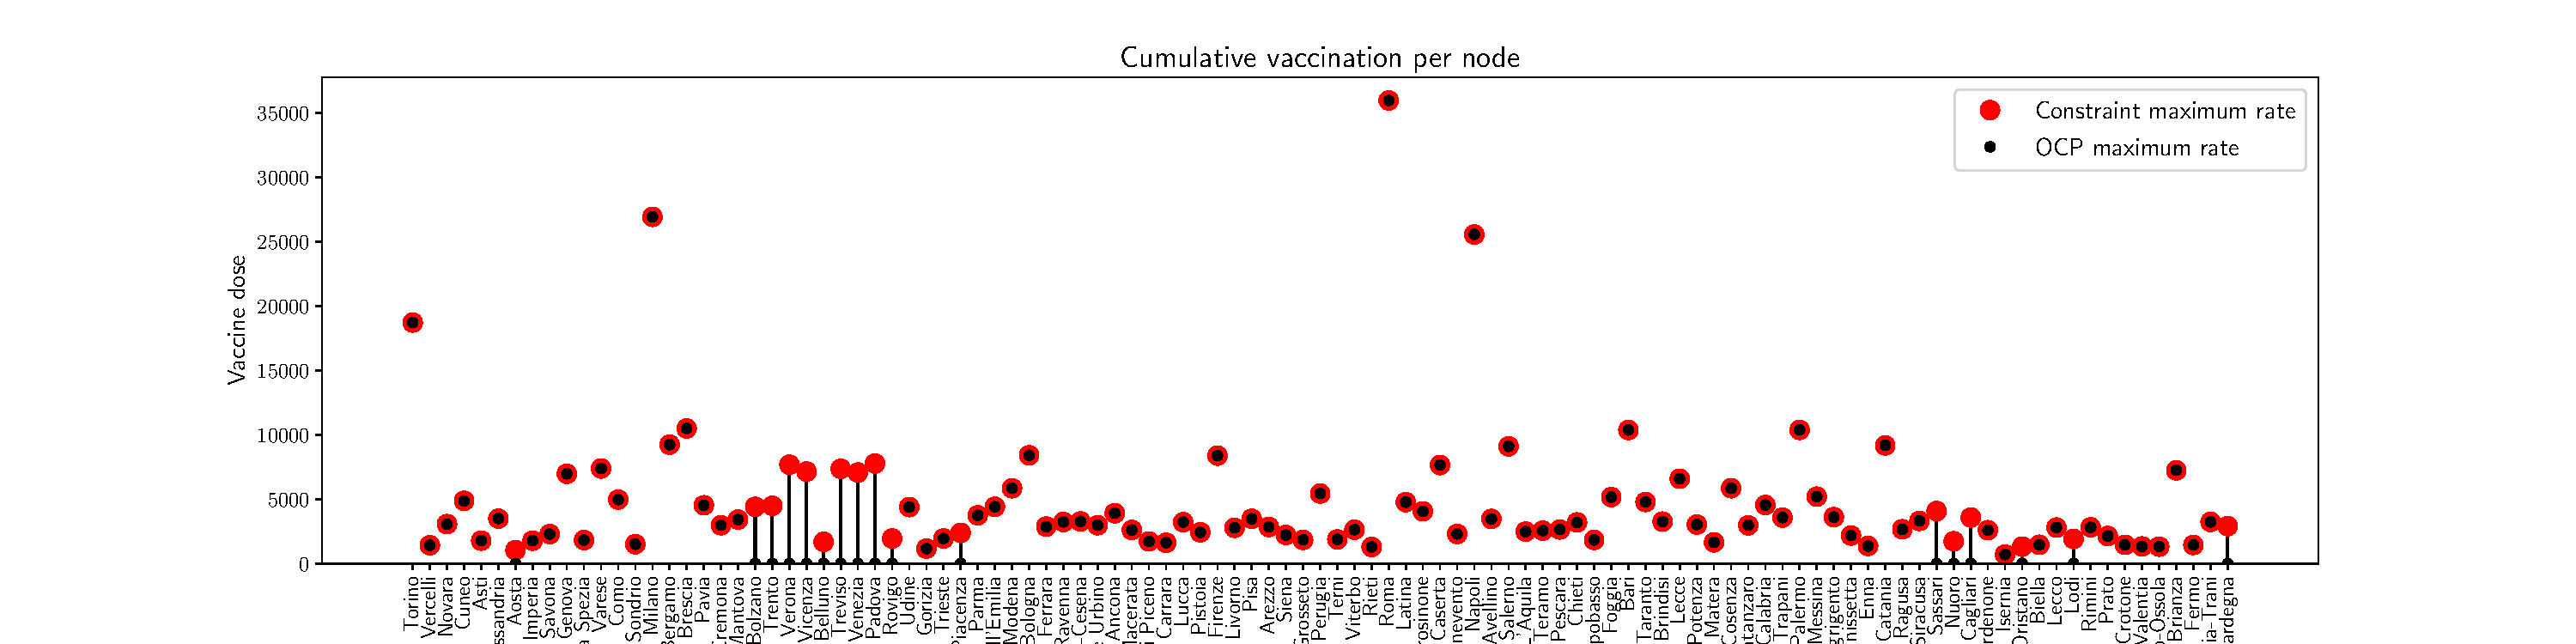
\includegraphics{fig_italy-ocp/figuresSI/SI_constraint_dist.pdf}
    \caption[Vizualisation of the local maximum vaccination rate constraint][-2\baselineskip]{Local maximum vaccination rate constraint $v_i^\mathrm{max}$ for each province. This logistic constraint bounds the maximum number of vaccines to 0.5M of doses per day, with a local rate that is proportional to the node population. Here the maximum vaccination rate for each province (the constraint the solution has to comply with) is shown in red, and the maximum rate prescribed by the optimal solution while simulating the pessimistic scenario with a stockpile delivery of 479'700 doses, in black. The optimal solution uses the maximal capacity of the logistic network, while respecting the constraint defined.}
    \label{fig:OC_logistic_constraints}
\end{figure}


 % Description:model
\subsection{Epidemiological model.} 
The optimal control framework may be used with any compartmental SARS-CoV-2 transmission model that can be approximated by ordinary differential equations. To demonstrate its usefulness, it is applied a complex model based on previous work that was aimed to describe the first wave of COVID-19 infections in Italy\parencite{Gatto:SpreadDynamicsCOVID19:2020,Bertuzzo:GeographyCOVID19Spread:2020}. 
%Incidence and deaths are projected using the spatially distributed epidemiological model devised by Gatto et \textit{al.}\cite{Gatto:SpreadDynamicsCOVID19:2020} and further improved by Bertuzzo et \textit{al.}\cite{Bertuzzo:GeographyCOVID19Spread:2020}. 

The proposed framework is constituted of two disease transmission models, one "true" model and a simplified one used for control:
\begin{itemize}
    \item The full model is a COVID-19 model, as designed in\cite{Gatto:SpreadDynamicsCOVID19:2020, Bertuzzo:GeographyCOVID19Spread:2020}. This model is ODE-based, includes full connectivity based on mobility data, and is implemented in MATLAB using the adaptive step ode45 integration scheme. Using data assimilation, the joint-posterior distribution is obtained for all parameters of this model. 
    \item The simplified model used for optimal control is an approximation of the above model, integrated using an explicit Runge-Kutta 4 method with fixed stepsize. The problem is simplified by limiting the connectivity to the largest mobility fluxes (see fig.~\ref{fig:model_description_network} and optimizing only one realization of the posterior. This model is implemented in Python with the CasADi library.
\end{itemize}

\paragraph{Model description}
The model subdivides the Italian population into its 107 provinces represented as a network of connected nodes. Each province has local dynamics describing the number of individuals present in each of the model compartments: susceptible $S$, exposed $E$, pre-symptomatic $P$ (incubating infectious), symptomatic infectious $I$, asymptomatic infectious $A$, hospitalized $H$, quarantined $Q$, recovered $R$, and dead $D$. A tenth compartment, vaccinated individuals $V$, is added to the original nine, as shown in fig.~\ref{fig:model_description_diag}.

\begin{marginfigure}
\centering
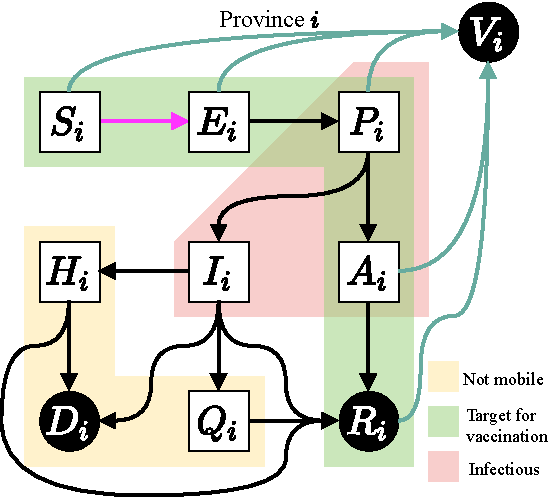
\includegraphics{fig_italy-ocp/figures/OCPItalydrawio2.pdf}
%    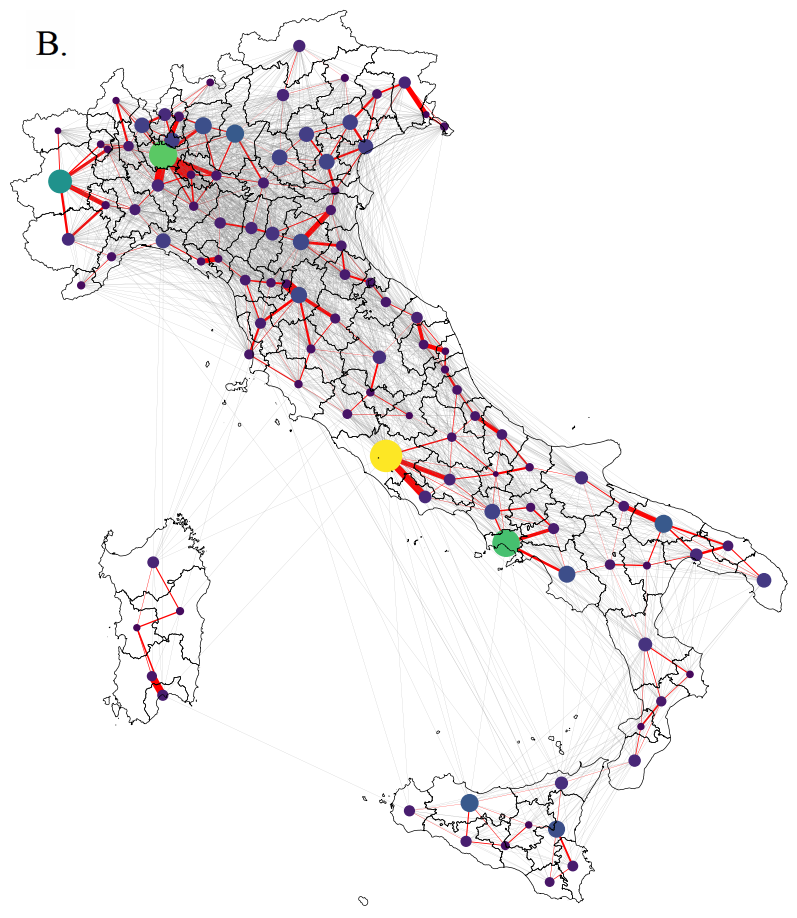
\includegraphics[width=0.40\textwidth]{fig_italy-ocp/figures/map_nd.png}
\margincaption[Optimal control model compartments diagram]{Diagram representing the compartments of the epidemiological model and the possible transitions in a single province. The control is the vaccination rate (teal arrows), aiming at minimizing incident infections (pink arrow). Individuals in compartments outside of the yellow block are able to move along the mobility network.}
    \label{fig:model_description_diag}
\end{marginfigure}


Apart from hospitalized $H$, quarantined $Q$, dead $D$, and symptomatic individuals $I$, a fraction of the other individuals commutes between provinces along the mobility network, thus node-to-node disease transmission is introduced along the network shown in fig.~\ref{fig:model_description_network}.

Compartments $P$, $A$, and $I$ have different degrees of infectiousness and contribute to the force of infection (Equation \eqref{eq:foiL} and \eqref{eq:foiM}), which represents the rate at which susceptibles $S$ become infected and, thus, enter the exposed compartment $E$. The force of infection in each province is constituted of a local and a mobility component. The local component describes transmission among the local individuals. The mobility component considers that local susceptibles may enter in contact with infected individuals that are traveling, and oppositely, susceptible commuters may become infected through contact with local infected. Connected provinces contribute to this process depending on the strength of the mobility fluxes from and to the node of interest.

The estimated vaccine efficacy and immunity duration depends on the vaccine type. Because the focus is on spatial patterns and differences among vaccination strategies, the vaccination process is simplifed by assuming a one-dose vaccine with instantaneous 100\% efficacy. %This simplification does not influence the relative vaccine allocation between provinces and is independent of the specific vaccine used. 
Moreover, that vaccines protection is assume persists during the three months of projection considered.

In the end, the COVID-19 transmission dynamics are described by the following set of ordinary differential equations in each node $i$: 
\begin{equation}\label{eq:sepiar}
\begin{split}
    \dot{S}_i &= - \lambda_i(t) S_i - r^v_i(t) S_i \\
    \dot{E}_i &= \lambda_i(t) S_i -  (\delta^E + r^v_i(t)) E_i \\
    \dot{P}_i &= \delta^E E_i -  (\delta^P+r^v_i(t))  P_i \\
    \dot{I}_i &= \sigma \delta^P P_i - (\gamma^I + \eta)  I_i \\
    \dot{A}_i &= (1 - \sigma) \delta^P P_i - (\gamma^A+ r^v_i(t)) A_i \\
    \dot{Q}_i &= \zeta \eta I_i - \gamma^Q Q \\
    \dot{H}_i &= (1-\zeta) \eta I_i - (\gamma^H + \alpha^H)H \\
    \dot{R}_i &= \gamma^I I_i + \gamma^A A_i + \gamma^H H_i + \gamma^Q Q_i - r^v_i(t) R_i\\
    \dot{V}_i &= r^v_i(t) \cdot (S_i + E_i + P_i + A_i + R_i).
\end{split}
\end{equation}
$N_i$ the population of province $i$. Susceptible individuals get exposed to the pathogen at rate~$\lambda_i(t)$, corresponding to the force of infection for community~$i$, thus becoming latently infected (but not infectious yet). Exposed individuals transition to the post-latent, infectious stage at rate~$\delta^E$. Post-latent individuals progress to the next infectious classes at rate $\delta^P$, developing an infection that can be either symptomatic---with probability~$\sigma$---or asymptomatic---with probability $1 - \sigma$. Symptomatic infectious individuals recover from infection at rate~$\gamma^I$ and may seek treatment at rate~$\eta$. Asymptomatic individuals recover at rate~$\gamma^A$.  Infected individuals who sought treatment are either hospitalized (rate $1-\zeta$) or quarantined (rate $\zeta$) at home and are considered to be effectively removed from the community, thus not contributing to disease transmission. Individuals who recover from the infection are assumed to have long-lasting immunity to reinfection at the timescale studied, but possible loss of immunity can be easily included in the model. Hospitalized individuals die at rate $\alpha_H$ and recover at rate $\gamma^H$.

Individuals in compartments $S, E, P, A, R$ might receive vaccine doses. If the chosen strategy allocates $v_{i}(t)$ doses in node $i$ at time t, the vaccination rate is

\begin{equation}
r^v_i(t) = \frac{v_{i}(t)}{S_i(t) +  E_i(t) + P_i(t) + A_i(t) + R_i(t)}
\end{equation}

Vaccinated individuals are moved at rate $r^v_i(t)$ from their original compartments to compartment $V$, where they do not contribute to the infection anymore.

\paragraph{Force of infection and simplifications}
The force of infection of the full model is specified as in Gatto et \textit{al.}\cite[-4\baselineskip]{Gatto:SpreadDynamicsCOVID19:2020}, Bertuzzo et \textit{al.}\cite{Bertuzzo:GeographyCOVID19Spread:2020}. In addition to province's local dynamics, it also considers that local susceptibles may enter in contact with infected individuals that are traveling, and oppositely, susceptible commuters may become infected through contact with local infected. The force of infection of the OCP model slightly simplified:

The force of infection $\lambda_i(t)$ is split between the sum of the local force of infection $\lambda^L_i(t)$, from infected in node $i$ and a mobility-driven force of infection from the network $\lambda^N_i(t)$, hence $\lambda_i(t) = \lambda^L_i(t) + \lambda^M_i(t)$. While running our model, it became apparent that $\lambda^M_i(t) \ll \lambda^L_i(t)$. Hence this artificial separation will be exploited when simplifying our model. As described below, $\lambda^M_i(t)$ is updated every day whereas $\lambda^L_i(t)$ is updated at each integration step.
\begin{marginfigure}
\centering
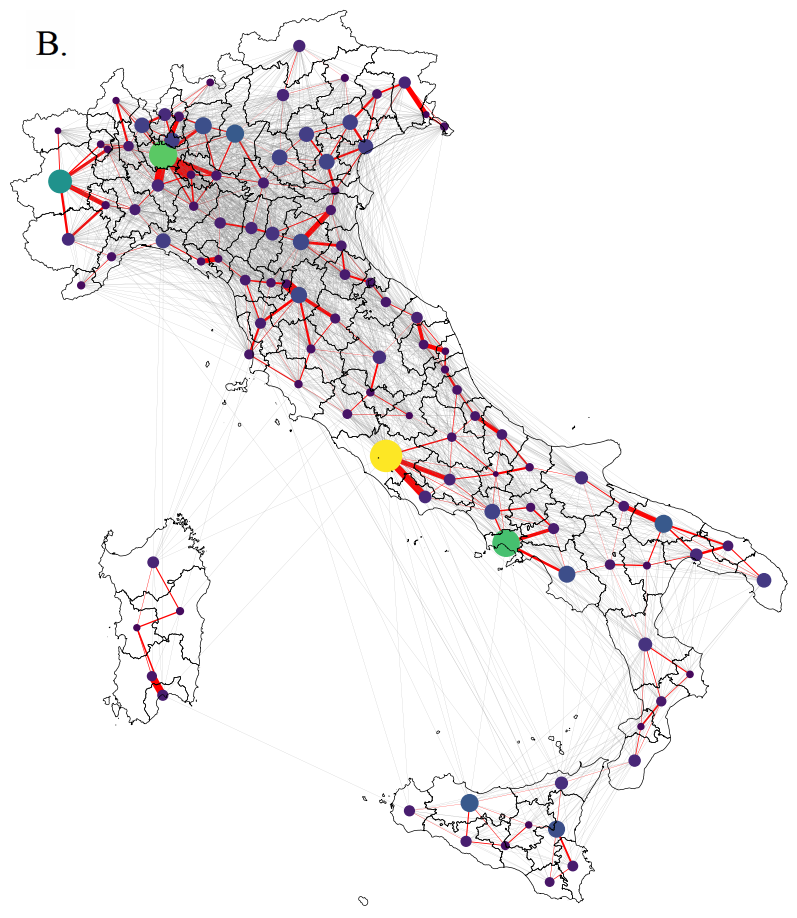
\includegraphics{fig_italy-ocp/figures/map_nd.png}
\margincaption[Optimal control mobility network]{Mobility network: the force of infection in a province is coupled to the dynamics of other connected provinces. To reduce the problem to a tractable size, only the most important connections (red edges) are considered when optimizing, but the full network (red and grey edges) is used to assess our strategies. Nodes size and color display each province's population, and edges width shows the straight of the coupling between each pair of provinces.}
    \label{fig:model_description_network}
\end{marginfigure}

As for the formulations of the force of infection, the formulas designed by \textcite{Gatto:SpreadDynamicsCOVID19:2020,Bertuzzo:GeographyCOVID19Spread:2020}are recalled here. The local force of infection reads:
\begin{equation} 
     \lambda^L_i(t) = C_{i,i} \beta_{0}  \beta_i(t) \cdot \frac{C_{i,i}  (P_i + \epsilon_A  A_i) + \epsilon_I  I_i}{C_{i,i} \cdot (S_i + E_i + P_i + R_i + A_i + V_i) + I_i}, \label{eq:foiL}
\end{equation}
and the influence of other provinces on province $i$ is written as:
\begin{equation}
     \lambda^M_i(t) = \sum_{m, m \neq i} \left( 
     C_{i,m} \cdot 
     \frac{
     \sum_{n, n \neq m} \left[ C_{n,m} \cdot \beta_{0}  \beta_n(t)  (P_n + \epsilon_A  A_n) \right] + \epsilon_I  \beta_{0}  \beta_m(t)  I_m
     }
     {
     \sum_{l, l \neq m}  \left[C_{l, m} \cdot (S_l + E_l + P_l + R_l + A_l + V_l) \right] + I_m
     } 
     \right), \label{eq:foiM}
\end{equation}
where $\beta_{0}$ is the baseline transmission rate, while $\beta_{i}(t)$ is a spatially distributed and time-varying parameter describing site- and time-specific variations in transmissibility due to non-pharmaceutical interventions or other exogenous factors like variants. The parameters $\epsilon_A$ and $\epsilon_I$ represent the reduction of transmission respectively for asymptomatic and symptomatic individuals with respect to pre-symptomatic individual transmissions. Matrix $C$ accounts for mobility: each element $C_{i,j}$ of the matrix ($i \neq j$) represents the proportion of individuals moving from $i$ to $j$, while the diagonal elements $C_{i,i}$ are the proportions of individual who do not move in each node $i$.

The objective for our model is to minimize the total incidence of infections, i.e., $\int_{t_i}^{t_f} \sum_i \lambda_i(t) S_i$. Note that for the present model, this is equivalent to optimizing the total deaths or hospital admissions, as without risk-classes the sizes of these two compartments are proportional to each other.


\begin{figure}[!ht]%[width=0.75\textwidth]
    \centering
    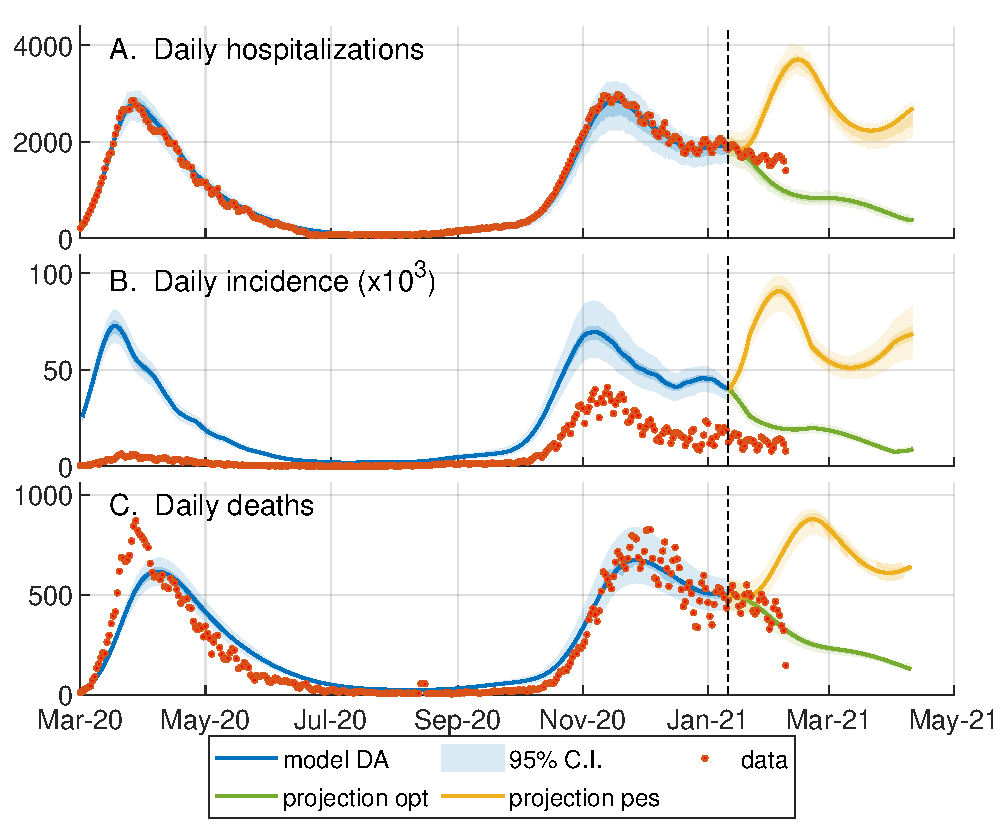
\includegraphics{fig_italy-ocp/figures/DA_italy1.pdf}
    \caption[Data assimilation and scenarios for optimization]{Data assimilation and scenarios for optimization. Comparison between the model outputs (95\% confidence interval (CI) of the ensemble, blue shaded area) and the corresponding epidemiological data from March 2020 to January 2021. The orange and green shaded area respectively show the ensemble dynamics (95\% CI) of what is called pessimistic and optimistic transmission scenarios from January to April. The optimal vaccination strategy in the optimistic (or pessimistic) scenario is computed with respect to the the continuous green (or orange) line, representing the model trajectory obtained using the median of each ensemble parameter. A. The data on the daily hospitalizations is estimated as described in \parencite{Bertuzzo:GeographyCOVID19Spread:2020}; this data at the regional level is assimilated on a moving window of 14 days to update the model parameters describing the local transmission rates (see SI). B. Daily number of newly exposed individuals versus the reported positive cases. Note that, the model assumes the presence of 90\% asymptomatics among the exposed individuals, who are possibly not detected by the surveillance system. C. Daily number of deaths. %\textbf{D.} Estimated reproduction number. The fluctuations during summer 2020 are mainly due to local outbreaks generated by  imported cases which cannot be directly considered in the model since the data is not public available.  
    }\label{fig:model_DA}
\end{figure}

\paragraph{Calibration and scenarios}The epidemiological model, previously calibrated during the first wave of COVID-19 in Italy\cite{Gatto:SpreadDynamicsCOVID19:2020,Bertuzzo:GeographyCOVID19Spread:2020}, is updated up to January 11, 2021 using an iterative particle filtering. This data assimilation scheme allows us to capture the second wave of infections that hit Italy in the Fall of 2020, a necessary requirement to generate model projections that take into account the whole epidemic history, as shown in fig.~\ref{fig:model_DA}. In our approach, model projections are described by an ensemble of a thousand trajectories associated with different parameters, whose distributions quantify the model uncertainty. 
\marginnote{The detailled methods for the data assimilation scheme is provided in the supplemental information of \parencites{Lemaitre:OptimizingSpatiotemporalAllocation:2021}, and this thesis focuses on the optimal control problem. However, data assimilation is a key compomentent allowing to update models states and parameters as new data becomes available, making it necessary of model predicitive control (see \textsc{Discussion and Conclusion}.}
Two projection scenarios are considered, each characterized by a possible rate of epidemic transmission, see fig.~\ref{fig:model_DA}. The "Optimistic" scenario assumes a constant lowering of transmission from January 11, 2021 to April 11, 2021; the "Pessimistic" scenario considers a gradual increase in transmission until mid February 2021, which results in a third wave. 

For each scenario, the optimal control problem is solved for one reference model trajectory, whose parameters and state on January 11, 2021 are obtained as the median values of the 1'000 model realizations. In this way, the reference trajectory approximately represents the ensemble median in each province. Then, the effectiveness of the optimal allocation is assessed on the full ensemble of trajectories.


%Note that, since this spatial model does not consider risk-classes, the vaccination strategy minimizing the incidence also minimizes deaths or hospitalizations.

This division is necessary in order to solve the optimal control problem (OCP) in a reasonable time. To adapt our framework to another model/country, one would need to update the "true" model to a suitable candidate (which could be a stochastic model, a Hidden Markov model, or any other kind) and design a tractable approximation of this new model to be solved by optimal control.

In order to evaluate the effectiveness of our approach, the optimal vaccination course that minimizes the objective is computed based on the simplified model. Then, this strategy and the alternative ones are evaluated on the full model, for different posterior realisations. If the simplified model is sufficiently accurate, the performance loss is small and the proposed strategy outperforms simpler strategies, as shown in our simulation results.

\subsection{Formulation of the optimal control problem}
\paragraph{Optimal control problem definition}Let $n$ the number of spatial nodes ($n=107$ provinces in Italy) and $m$ the number of epidemic states in our model ($m=9$ states).
The states of the system are noted $x(t) \in \mathbb{R}_+^{n\times m}$, i.e., $x(t)$ is a vector containing the epidemic variables $S_i(t)$, $E_i(t)$, $P_i(t)$, $I_i(t)$, $A_i(t)$, $Q_i(t)$, $H_i(t)$, $R_i(t)$, $V_i(t)$ for every province $i=1,...,n$. The rate of vaccine rollout for every node $i$ at time $t$ is written $v(t) = (v_1(t),...,v_n(t)) \in \mathbb{R}_+^{n}$, representing our control variable:. %Omitting the time dependence $t$, t

The dynamics of the epidemiological model (Equation~\eqref{eq:sepiar}) are expressed as an ordinary differential equation in each province $i$:
\begin{equation}
    \label{eq:sepiar_compact}
    \dot x_i(t) = F_i(x_i(t),v_i(t), m_i(t), t),
\end{equation}
where $m_i(t)$ carries the contribution of other provinces to the force of infection of node $i$. The epidemiological model can be described by the following system of ordinary differential equations coupling disease transmission among all provinces:

\begin{align}
    \dot x(t) = F(x(t),v(t),m(t),t)
    \label{eq:dynamics}
\end{align}

For simplicity, the time dependence is dopped in the equations below, and the state and control variables for the full system as
\begin{align*}
    x = (x_1,\ldots,x_n), && v = (v_1,\ldots,v_n),
\end{align*}
The global dynamics for all provinces are denoted:
\begin{equation*}
    F(x,v) = (F_1(x_1,v_1, m_1),\ldots,F_n(x_n,v_n, m_n)).
\end{equation*}
The coupled force of infection in node $i$ is denoted $\lambda_i$. The cost function is defined as the national incidence, i.e., the sum of new infections (transitions $S_i\longrightarrow E_i$) in all provinces at time $t$,  for every node $i$, i.e.,

\begin{equation*}
    L(x,v) = \sum_{i=1}^n \lambda_i S_i.
\end{equation*}

For the sake of generality the terminal cost $M$ is introduced, which can be used to ensure that the system is left in a proper state instead of optimizing for short-term gain. Since properly designing the terminal cost could require a long analysis, for simplicity it is not used in this work, hence $M(\cdot) = 0$.

Given our dynamical system with states $x$, controls $v$, and dynamics $F$, the OCP is:

\begin{subequations}
    \label{eq:ocp}
    \begin{align}
        \min_{v(\cdot)} \ \ & \int_{0}^{T} L(x(t),v(t)) \ \mathrm{d}t + M(x(T)) \\ \label{eq:ocp_dyn1}
        \mathrm{s.t.} \ \ & x(0) = \hat x_0, \\ \label{eq:ocp_dyn2}
        &\dot x(t) = F(x(t),v(t)), && \forall \, t\in[0,T], \\ 
        &H(x(t),v(t)) \leq 0, && \forall \, t\in[0,T],
    \end{align}
\end{subequations}

where the aim is to minimize the cost function over the control horizon $T$, while enforcing the modeled SARS-CoV-2 transmission dynamics (Equations \eqref{eq:ocp_dyn1} and \eqref{eq:ocp_dyn2}). Moreover, the constraints imposed by vaccine availability and the maximum vaccination rate are lumped in function $H$ that expands to
\begin{subequations}
    \begin{align}
        v_i(t) &\geq 0, && i\in\mathbb{I}_1^n, \label{eq:constr_vacc_met} \\
        \int_{t_\mathrm{d}}^{t_\mathrm{d}+1} v_i(t) \ \mathrm{d}t &\leq v_i^\mathrm{max} \propto N_i, && i\in\mathbb{I}_1^n,\ t_\mathrm{d} \in \mathbb{I}_0^T,  \label{eq:constr_day_met} \\
        \int_{0}^{t} \sum_{i=1}^n v_i(t) \ \mathrm{d}t &\leq D(t), && \forall \, t\in[0,T], \label{eq:constr_week_met}
    \end{align}
\end{subequations}

where time is measured in days, and $\mathbb{I}_a^b$ is the set of all integers $a\leq k\leq b$. Equation \eqref{eq:constr_vacc_met} enforces that one can only distribute a non-negative amount of vaccine doses. Equation \eqref{eq:constr_day_met} states the logistic constraints, which limit to $v_i^\mathrm{max}$ the amount of individuals that can be vaccinated each day in each node; here $t_\mathrm{d}$ is the time at which each day starts. The daily vaccination capacity of each province is set to be proportional to its population size $N_i$, assuming a fair distribution of the sanitary infrastructure among provinces, as shown in SI (Figure \ref{fig:OC_logistic_constraints}). The constraint on the national stockpile is materialized by Equation
\eqref{eq:constr_week_met}, which ensures that the total vaccine allocation across all nodes does not exceed the stockpile $D(t)$. The stockpile is replenished every Monday by the delivery of new vaccines, hence $D(t)$ is a staircase function.



\paragraph{Transforming the optimal control problem into a non-linear programming problem}

\marginnote[1\baselineskip]{For an overview of the possible solution approaches for optimal control problems the interested reader is refered to \textcite{Betts:PracticalMethodsOptimal:2010,Biegler:NonlinearProgramming:2010}. In particular, in this work, a variant of direct multiple shooting \textcite{Bock:MultipleShootingAlgorithm:1984} tailored to distributed systems \textcite{Savorgnan:MultipleShootingDistributed:2011} is used.} 

The optimal control problem in Equation~\eqref{eq:ocp} is solved by a direct method, also called \emph{first discretize, then optimize}, which transforms the control problem into a nonlinear programming problem. Within direct methods, direct multiple shooting is employed. 


Our time window $[0,T]$ is divided into a uniform time grid $t_0,\ldots,t_N$, with $N+1$ points and $t_0=0$, $t_N=T$. Hence there are $N$ intervals $[t_k,t_{k+1}]$, and the states at time $t_k$ is denoted $x_k=x(t_k)$, and $v_k$  represent the controls in interval $[t_k,t_{k+1}]$. The control function is parameterized using basis functions with local support. \marginnote[-2.5\baselineskip]{For discretization, a uniform time grid is choosen here, i.e., $t_{k+1}=t_k+\delta_t$ and a piecewise constant control function, i.e., $v(t)=v_k$, $t\in [t_k,t_{k+1}]$. This is a common choice but other are possible. Here $\delta t=1\ \mathrm{day}$.}

The continuous-time dynamics~$F$ in Equation \eqref{eq:dynamics} are transformed by numerical integration into the discrete-time operator $f$ by numerical integration. The system dynamics are then discretized to obtain a discrete-time system.

\begin{align*}
    x_{k+1} = f(x_k,v_k),
\end{align*}

satisfying $x_k=x(t_k)$ for all $k=0,\ldots,N$. Moreover, the cost function is also discretized, to obtain

\begin{align*}
    l(x_k,v_k)=\int_{t_k}^{t_k+1} L(x(t),v(t)).
\end{align*}

The discretization is performed using numerical integration techniques (such as a fourth-order Runge-Kutta scheme, with 50 steps per days) to obtain a good approximation of the true trajectory and cost. Finally, the path constraints $H$ are relaxed and imposed at a finite amount of time instants, here coinciding with the time grid $t_0,\ldots,t_N$. Since in our case the constraints only involve the controls, no approximation is introduced by enforcing these constraints only on this uniform grid. The OCP~\eqref{eq:ocp} is then approximated by the nonlinear programming problem

\begin{subequations}
    \begin{align}
        \min_{x,v} \ \ & M(x_N)+\sum_{k=0}^{N-1} l(x_k,v_k)  \\ 
        \mathrm{s.t.} \ \ & x_0 = \hat x_0 \\
        & x_{k+1} = f(x_k,v_k), && k\in \mathbb{I}_0^{N-1}, \\
        &H(x_k,v_k)\leq 0, && k\in \mathbb{I}_0^{N-1}.
    \end{align}
        \label{eq:ocp_nlp}
\end{subequations}
\marginnote[-7\baselineskip]{%In~\eqref{eq:ocp_nlp}, 
Here both the states $x=(x_0,\ldots,x_N)$ and the controls $v=(v_0,\ldots,v_{N-1})$ are defined as optimization variables, which is a distinguishing trait of multiple shooting as opposed to single shooting.}

The force of infection associated with mobility is assumed to constant over each day. Thus, each node dynamics can be made independent of the other nodes dynamics by introducing an auxiliary control variable $z$ that is constrained to match the force of infection due to the other nodes at the beginning of each time interval. Then, the dynamics of the decoupled system in each node can be written as:

\begin{align*}
\dot x_i(t) &= F_i(x_i(t),z_{i,k}), && t\in[t_k,t_{k+1}] \\
x_i(t_k) &= x_{i,k} + g_i(v_{i,k}), && z_{i,k} = e_i(x).
\end{align*}

\paragraph{Solving the Non-linear programming problem} Nonlinear programming problems may be solved by readily available solvers using the primal-dual interior point method. The main difficulty in solving the proposed nonlinear programming problem \eqref{eq:ocp_nlp} is the large dimension of the system and the non-linearities of the model. In order to bring the problem to a tractable form, three simplifications are introduced: (a) vaccines are administered instantaneously at the beginning of each day, rather than with a constant rate over the whole day; (b) the component of the force of infection taking into consideration the mobility of individuals across provinces is evaluated at the beginning of each day and remains constant through the day; and, (c) the mobility network is simplified, by keeping only the most important connections (see fig.~\ref{fig:model_description_network}), thus increasing the sparsity of the underlying spatial connectivity matrix. These simplifications deliver a significant computational advantage, and the impact on the model  accuracy was verified to be limited. 
\marginnote[-11\baselineskip]{Note that, even if the optimal strategy is computed using the simplified model, its impact in terms of averted cases and deaths is evaluated using the full epidemiological model without any of these simplifications. A more detailed discussion on this subject, and on the impact of the simplification is given in the \textsc{Appendix to Chapter 7}.}
\marginnote[-2\baselineskip]{The full framework and analysis code is available here: \url{https://github.com/jcblemai/COVID-19_italy-vaccination-oc}.} 
The nonlinear programming problem arising from the simplified epidemiological model is non-convex, and involves approximately $10^{5}$ variables and $10^5$ constraints. The problem is formulated within the automatic differentiation framework CasADi\cite{Andersson:CasADiSoftwareFramework:2018} and solve it using Ipopt~\cite{Wachter:ImplementationInteriorpointFilter:2006} with the HSL ma86 large sparse symmetric indefinite solver\cite{HSLCollectionFortran}, which exploit the sparsitity of the problem. 
Solving the OCP is both CPU and RAM intensive. Numerical computations are preformed on the Helvetios cluster the EPFL HPC facility (one problem per computing node, each equipped with 36 2.3 GHz cores and 192 GB RAM). On this cluster, it takes approximately four days to solve the large-scale OCP just presented. It should be possible to solve even larger problems with more RAM available. 


%% ***********************************************************************************************
\section{Results}
%% ***********************************************************************************************
Using state-of-the-art linear algebra solvers and automatic differentiation, each scenario (optimistic and pessimistic, with different weekly stockpile deliveries) is solved for the optimal vaccination allocation. The optimal vaccination strategies are obtained for a set of eight scenarios drawn from the spatial model from January 11, 2021 to April 11, 2021. These scenarios are a combination of two projection scenarios (pessimistic vs optimistic) and four assumptions on the weekly stockpile delivery (479'700, 1M, 1.5M or 2M doses delivered per week). In each scenario, the optimal solution is a spatially explicit vaccine roll-out policy, i.e. an indication of the number of vaccine doses to be deployed in each province each day. 
%% ***********************************************************************************************
\subsection*{Comparison of vaccination strategies}
In order to measure the potential impact of the optimal allocation strategy, it is compared against three non-optimized, yet reasonable alternative approaches: vaccinate proportionally to the future incidence as projected by the epidemiological model; vaccinate proportionally to the number of susceptible individuals in each province; vaccinate proportionally to the province's population. 
Comparisons with additional alternative strategies are presented in SI. Spatial prioritization based on epidemiological criteria, such as past\cite{Lee:AchievingCoordinatedNational:2020} or future\cite{Pasetto:RealtimeForecastingCholera:2018} incidence, has been thoroughly used in real campaigns and prospective studies.

For each of the eight scenarios considered, the number of averted infections is computed with respect to a zero-vaccination baseline, and the number of averted infections per vaccination dose (see Table \ref{table:averted_abs}). In the optimistic transmission scenario, characterized by a recess of the epidemic, the vaccination campaign has a lower impact on the averted infections per dose as only a small percentage of the vaccinated individuals would have been at risk of transmission. Obviously, the impact of the vaccination campaign is more evident in the pessimistic scenario where, for all strategies, the averted infections are larger than the vaccines deployed due to indirect protection effects. By virtue of the law of diminishing returns, the number of averted infections per dose decreases when increasing the stockpile. 

\begin{table*}[h!]
\centering
\begin{tabular}{clrrrr}
\toprule
Weekly stockpile& {} & \multicolumn{2}{c}{Averted Infections} & \multicolumn{2}{c}{Averted Infections} \\
delivery&  {}  &\multicolumn{2}{c}{(Millions)} & \multicolumn{2}{c}{ per doses} \\
& Method &  Optimistic & Pessimistic &     Optimistic & Pessimistic \\
\midrule
2 millions & \textsc{Optimal} &   $6.98$ &  $30.6M$ & $0.268$ & $1.18$ \\
        & Incidence &   6.32 &    28.1 &          0.243 &        1.08 \\
        & Population &   6.02 &    26.8 &          0.231 &        1.03 \\
        & Susceptibility &   5.97 &    26.7 &          0.229 &        1.02 \\
1.5 millions & \textsc{Optimal} &   $5.52$ &   $24.1$ &  $ 0.283$ & $1.24$ \\
        & Incidence &   4.89 &    21.7 &           0.25 &        1.11 \\
        & Population &   4.57 &    20.4 &          0.234 &        1.05 \\
        & Susceptibility &   4.51 &    20.3 &          0.231 &        1.04 \\
1 million & \textsc{Optimal} &    $3.9$ &    $16.9$ &  $0.3$ & $1.3$ \\
        & Incidence &   3.41 &    15.1 &          0.262 &        1.16 \\
        & Population &   3.08 &    13.8 &          0.237 &        1.06 \\
        & Susceptibility &   3.02 &    13.7 &          0.232 &        1.05 \\
479'700 & \textsc{Optimal} &  $2.01$ &  $8.54$ & $0.322$ & $1.37$ \\
        & Incidence &   1.73 &    7.57 &          0.278 &        1.21 \\
        & Population &   1.49 &    6.74 &          0.239 &        1.08 \\
        & Susceptibility &   1.43 &    6.54 &          0.229 &        1.05 \\
\bottomrule
\end{tabular}

\caption[Averted infections per dose for different allocation strategies]{Absolute number of averted infections and averted infections per dose during the first three months of 2021 as evaluated for the reference trajectory (see fig.~\ref{fig:model_DA}, and fig.~\ref{fig:OC_comparison} for an assessment on a set of trajectories drawn for the posterior distribution). The first column represents the considered scenarios of weekly stockpile replenishment, i.e.~the number of doses delivered to Italy every week, ranging from 479'700 to 2M.}
\label{table:averted_abs}
\end{table*}
\begin{figure}[!ht]
    \centering
    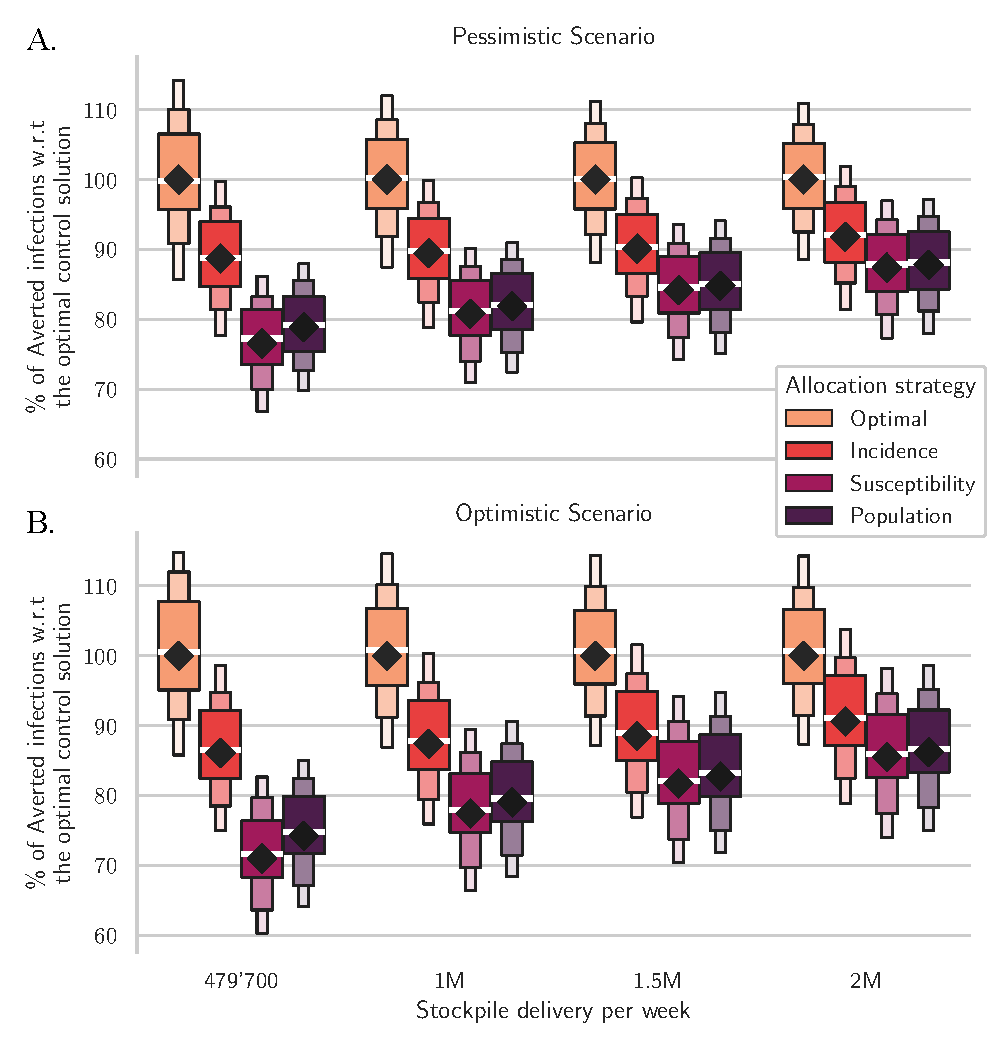
\includegraphics[width=\textwidth]{fig_italy-ocp/figures/scenarios_perturb_all.pdf}
    \caption[Comparison between different vaccine allocation strategies]{Comparison between different vaccine allocation strategies. Percentage of averted infections per vaccine doses from January 11, 2021 to April 11, 2021 resulting from province-scale vaccine allocation strategies for both the pessimistic (panel A) and the optimistic (panel B) scenarios based on: the optimal solution, population, proportion of susceptible individuals, and projected incidence (see color codes in the legend). The vaccine allocation is optimized for a (median) reference trajectory (diamonds), and assess the performance of the computed vaccination strategy over the whole posterior (box plots). For each projection scenario, results are normalized by the number of averted infections in the reference solution (see Table \ref{table:averted_abs} for absolute values). Results for alternative scenarios and vaccination strategies are shown in fig.~\ref{fig:OC_comparison_all}.}
    \label{fig:OC_comparison}
\end{figure}
The optimal solution always outperforms all alternative strategies in terms of the number of averted infections and in terms of averted infections per dose (see again Table \ref{table:all_strat}). Incidence-based allocation comes second, while population and susceptibility-based allocation are distant third and fourth respectively. The improvement between optimal and incidence-based allocation is significant, ranging from 8.8\% (pessimistic, 2M doses/week) to 16.2\% (optimistic, 479'000 doses/week). In fig.~\ref{fig:OC_comparison}, the black diamonds represent the percentage of adverted infections obtained using each strategy for the reference trajectory, with respect to the averted infections resulting from the optimal strategy. The optimal strategy is observed to have the largest relative benefits for the smallest stockpile in both the optimistic and pessimistic scenarios. 

In the pessimistic scenario (see fig.~\ref{fig:OC_comparison}.A), when 479'700 doses are made available each week, the averted infections associated with the optimal strategy in the reference projection are 1.37 per dose: $25~\%$ more compared to the strategies based on population or susceptible distributions (1.08 averted infections per dose), and more than $10~\%$ higher compared to the strategy based on the projected infections (1.21 averted infections per dose). These differences are smaller but still significant when increasing the weekly stockpile deliveries up to 2M doses; similar results are obtained also for the optimistic transmission scenario (Figure \ref{fig:OC_comparison}.B). 

The optimal control strategy considered here is computed for a reference model trajectory, which is the median of an ensemble of 1000 realizations. To further investigate the effectiveness of the optimal solution, it is applied to a subset of trajectories randomly sampled from the ensemble. The box plots in fig.~\ref{fig:OC_comparison} display the main quantiles of the averted infections computed for the ensemble of trajectories. The optimal strategy still yields better results than the ensemble of projections related to the other strategies, thus suggesting that the computed solution is robust even under the presence of perturbations in the forecasts of the epidemic dynamics. More importantly, for each realization of the ensemble and for each projection scenario, the optimal strategy systematically averts more infections than any of the other control strategies.

Our results suggest that it is possible to considerably increase the impact of vaccination campaigns by optimizing the vaccine allocation in space and time. For this task, optimal control provides the best possible strategy and sets a benchmark for the theoretical potential of a vaccination campaign.

%% ***********************************************************************************************
\subsection*{Analysis of the optimal vaccine allocation}

\begin{figure}[!ht]
    \centering
    %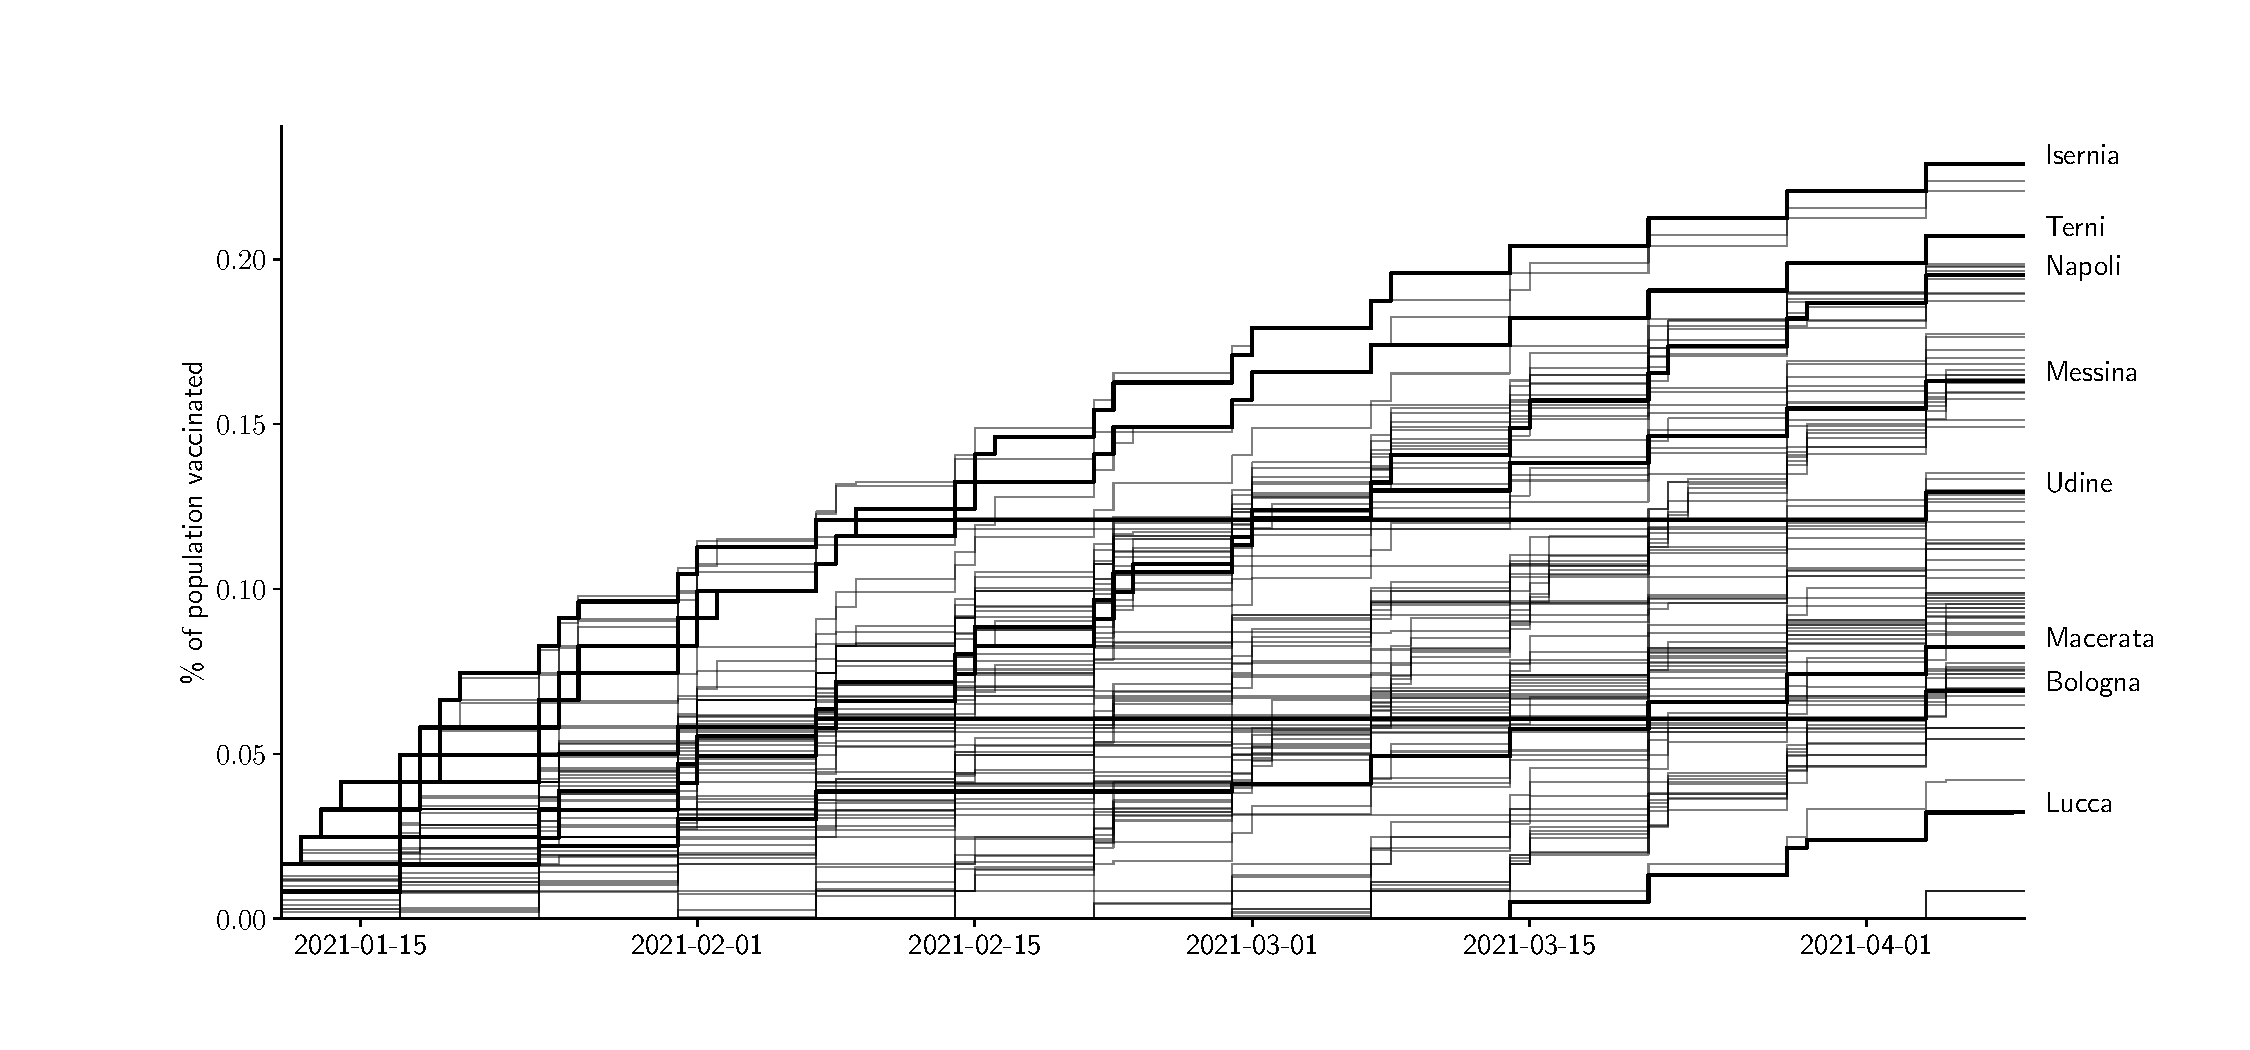
\includegraphics[scale=0.23]{figures/ts_optimal_selected.pdf} \\
    %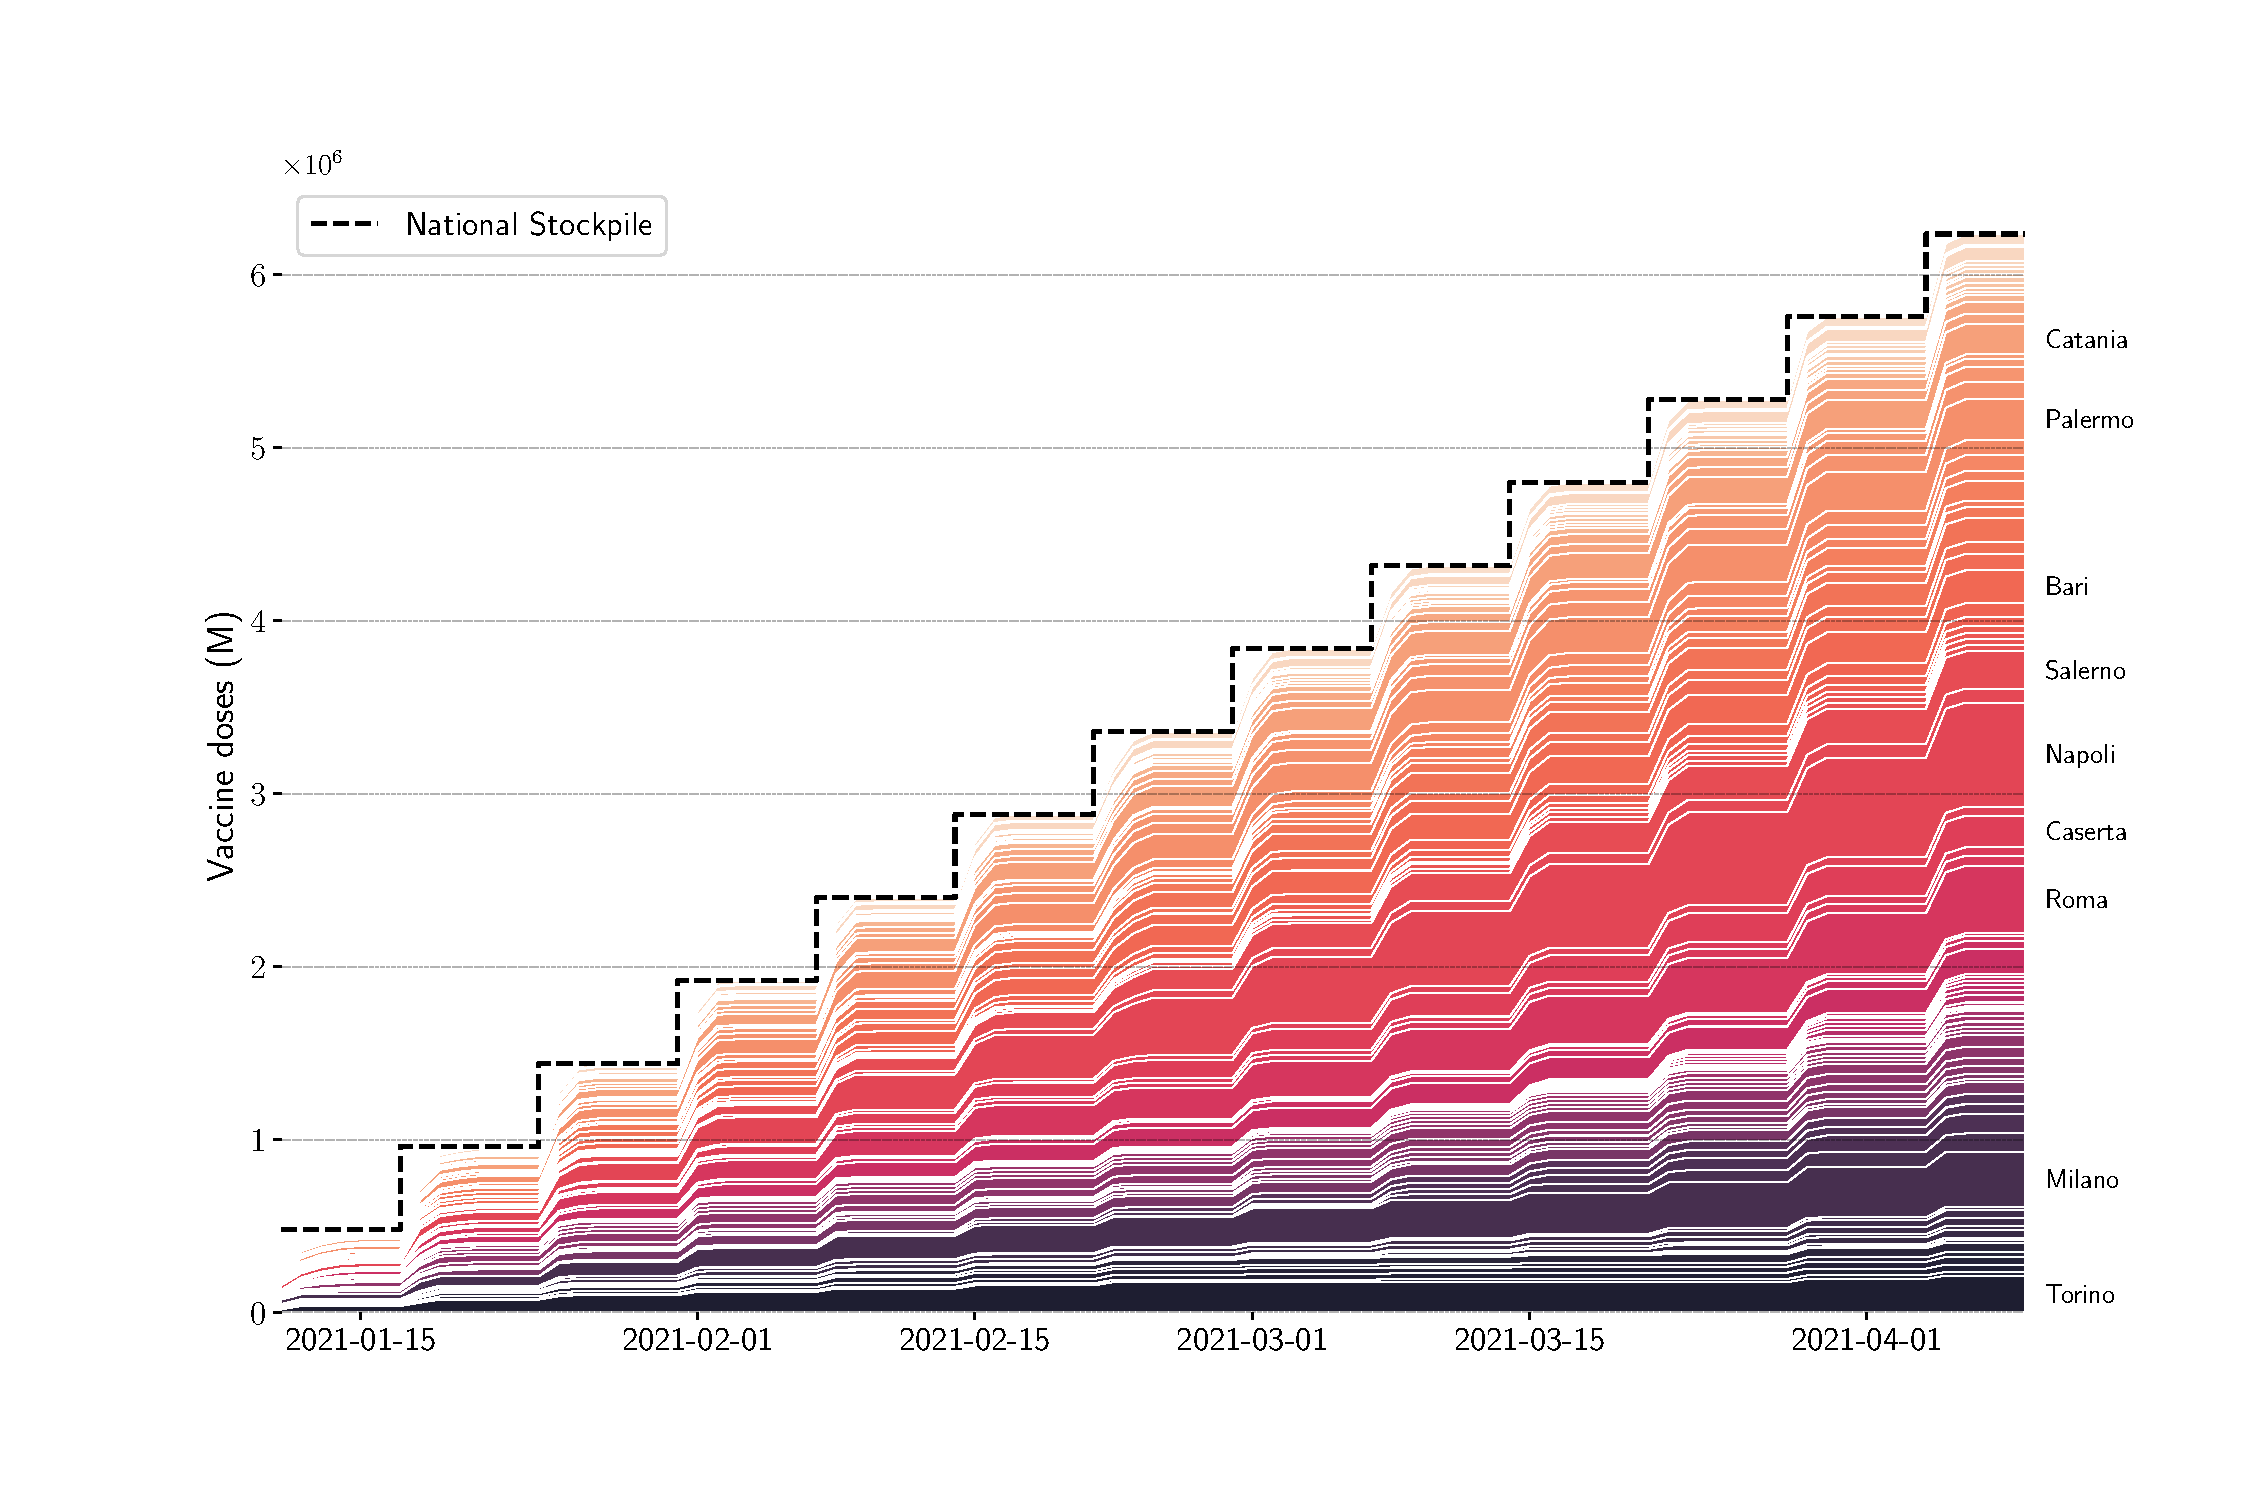
\includegraphics[scale=0.23]{figures/ts_optimal_stackplot.pdf}
    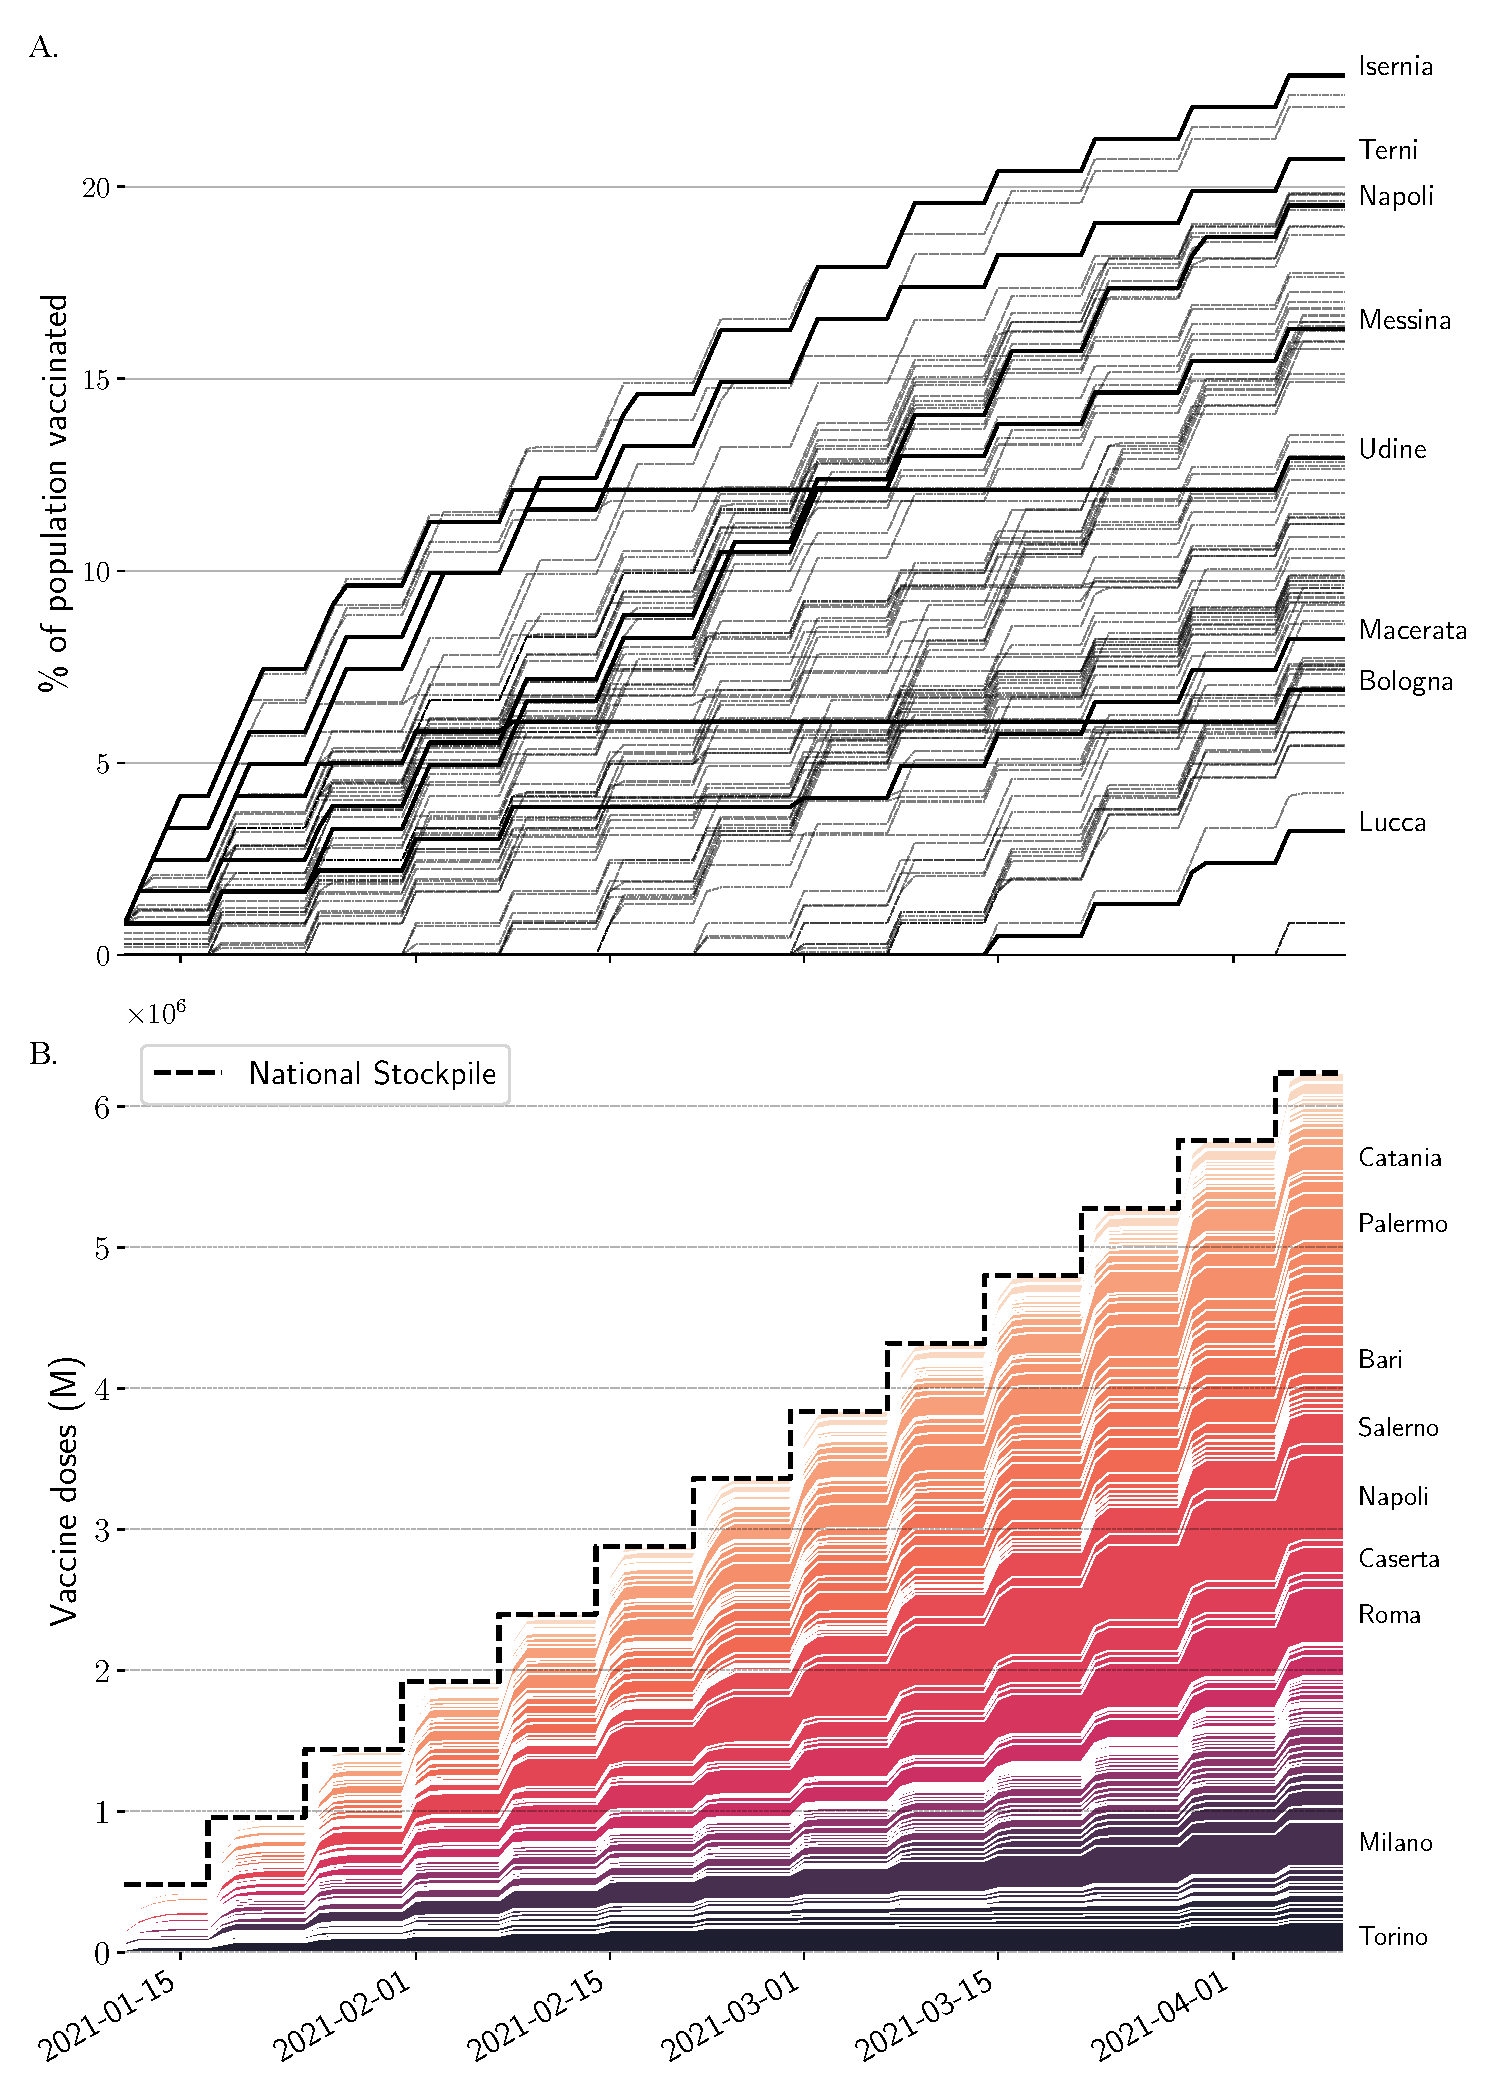
\includegraphics[width=\textwidth]{fig_italy-ocp/figures/ts_both.pdf}
    \caption[Optimal vaccine allocation for the baseline, pessimistic scenario. ]{Optimal vaccine allocation for the baseline, pessimistic scenario. \textsc{A.} Cumulative proportion of vaccine doses administered in the 107 provinces, (some of which are highlighted) . The local distribution rate is limited by a rate that is proportional to population. This logistic constraint is visualized here as the maximum slope, equal for every province.
    \textsc{B.} Stacked cumulative absolute number of vaccines in the 107 provinces of Italy. The national stockpile is shown in black, and is replenished every week (say on Mondays) with 479'700 doses. The name of the provinces with a final allocation of more than 150'000 doses is shown on the right.}
    \label{fig:OC_stackplot}
\end{figure}

The optimal vaccine allocation obtained as the solution of the optimal control framework is complex to analyze.%, and w- ought to do that by unraveling the mechanism behind its performance.
The strategy must obey the imposed logistic and supply constraints: 1) The vaccine stockpile is replenished every Monday by a fixed amount of doses (e.g., 479'700 doses in the baseline scenario), and 2) the maximum possible distribution capacity per province is limited, proportionally to the node population, so that the number of doses distributed across the country can be of 0.5M per day at maximum (more details in SI fig.~\ref{fig:OC_logistic_constraints}). \begin{marginfigure}[-10\baselineskip]
    \centering
    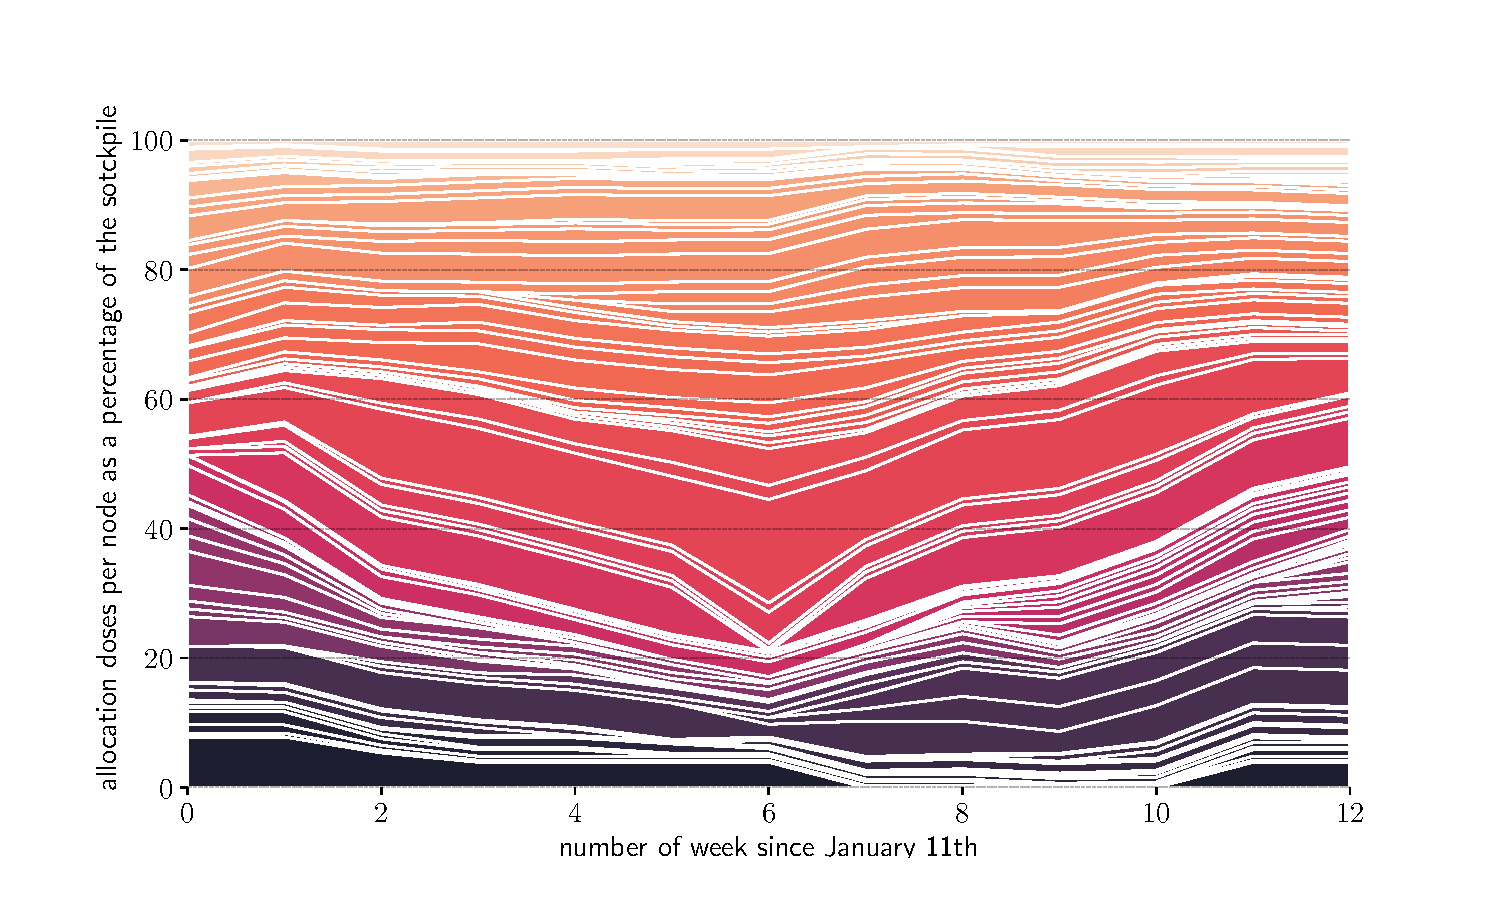
\includegraphics{fig_italy-ocp/figuresSI/SI_ts_optimal_stackplot_proportional.pdf}
    \margincaption[Time allocation for the pessimistic scenario]{Time allocation for the pessimistic scenario with a stockpile delivery of 479'700. Each week, the 479'700 doses are spread accross the provinces. This view unravel the temporal pattern in the allocation.}
    \label{fig:OC_temporal_alloaction}
\end{marginfigure}

The optimal vaccination course in time for the pessimistic, 479'700 doses/week scenario is shown in fig.~\ref{fig:OC_stackplot}. The optimal allocation respects is observed the two constraints on distribution (Figure \ref{fig:OC_stackplot}, A) and supply (Figure \ref{fig:OC_stackplot}, B). Moreover no province is vaccinated at the maximum possible rate during the whole campaign, and that provinces display a variety of vaccination patterns. Last, note that the vaccines received every Monday are always distributed during the following week, but that the rate of delivery on a national level increases with time (Figure \ref{fig:OC_stackplot}, B). Surprisingly, the optimal solution favors precise targeting over speed of delivery, in order to allocate more doses to those provinces where the impact of vaccines on the whole system is projected to be higher. Hence, in order to control infections, precise targeting may trump delivery speed. 

\begin{figure*}[!ht]
    \centering
    \includegraphics[width=1.1\textwidth]{fig_italy-ocp/figures/map_all.pdf}
    \caption[Spatial vaccine distribution patterns]{Spatial vaccine distribution patterns for the optimal allocation (left) and alternative strategies based on population, incidence and susceptibility (additional alternative strategies are presented in the \textsc{Appendix}). For each province and strategy is shown: the proportion of vaccinated individuals (top), the number of averted infections per inhabitant with respect to a no vaccination baseline (middle), and the proportion of individuals who are still susceptible at the end of the control horizon (bottom). Visual inspection suffices to reveal that the optimal allocation strategy is more alike the incidence-based allocation, but with vaccine doses spread-out to more provinces.}
    \label{fig:OC_multimap}
\end{figure*}

Furthermore, in the optimal solution every time a province is vaccinated, the rate of vaccination is equal to the maximum rate allowed by the local logistic constraint. This property is common to the alternative vaccination strategies, hence the difference in performance is due to the spatial allocation patterns.% of the optimal strategies provide the edge over the other strategies. 
In fig.~\ref{fig:OC_multimap}, one can already see by visual inspection that the optimal allocation distributes most of the available doses on a few provinces with high incidence. These provinces are neither the most connected nor the most populous in Italy. The optimal strategy makes then use of the information on the network connectivity to fine-tune the allocation, and deploys the vaccination on more provinces than the incidence-based strategy. %These little optimizations add up to the significant improvement seen above.

To further investigate these patterns, in fig.~\ref{fig:OC_scatter}.A is shown the number of administered doses vs the incidence projected without vaccines (the proxy variables leading to the second-best control performance), both normalized according to the resident population in each province. Sn allocation pattern whereby provinces with a higher incidence receive more vaccines is observed. However, the allocation is non-linear with respect to the projected incidence, suggesting that to better control the epidemic, the optimal allocation strategy takes into account other factors such as the importance of each province within the mobility network, as well as the proportion of susceptibles. When the weekly stockpile delivery is increased, as shown in fig.~\ref{fig:OC_scatter}.B, this pattern shifts to the right while remaining qualitatively consistent. Hence, the optimal allocation strategy is robust with respect to the overall vaccine availability constraint, and the same nodes are prioritized. Scatter plots with other covariates are shown in SI (Figures \ref{fig:OC_scatter_optimistic}--\ref{fig:OC_scatter_optimistic}). 

\begin{figure}[!ht]
\centering
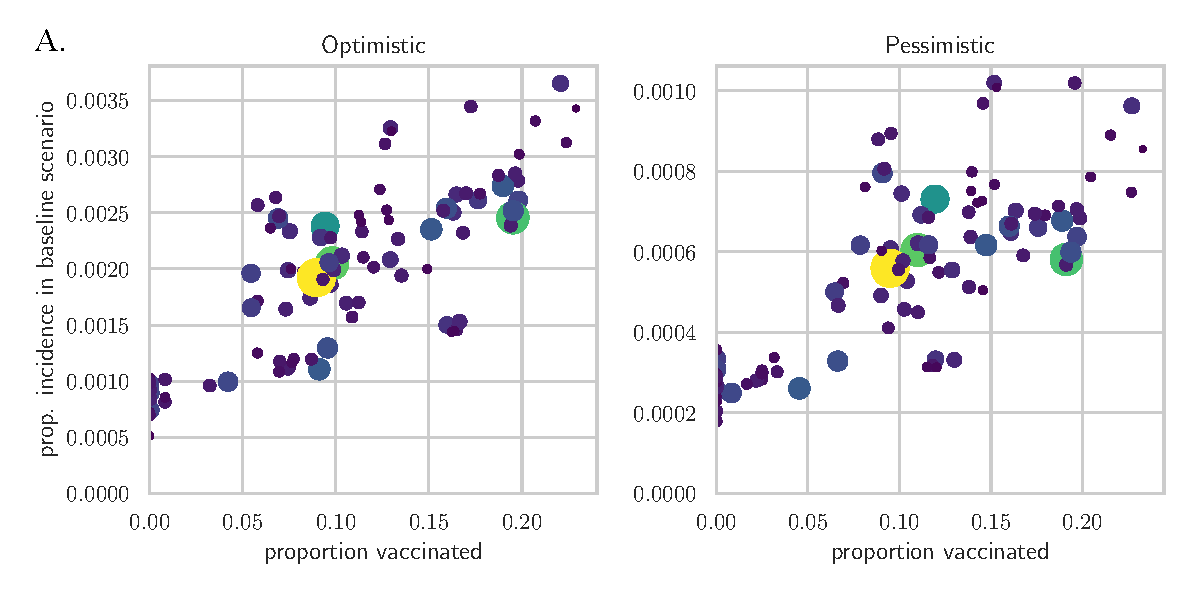
\includegraphics{fig_italy-ocp/figures/scatter_top.pdf}
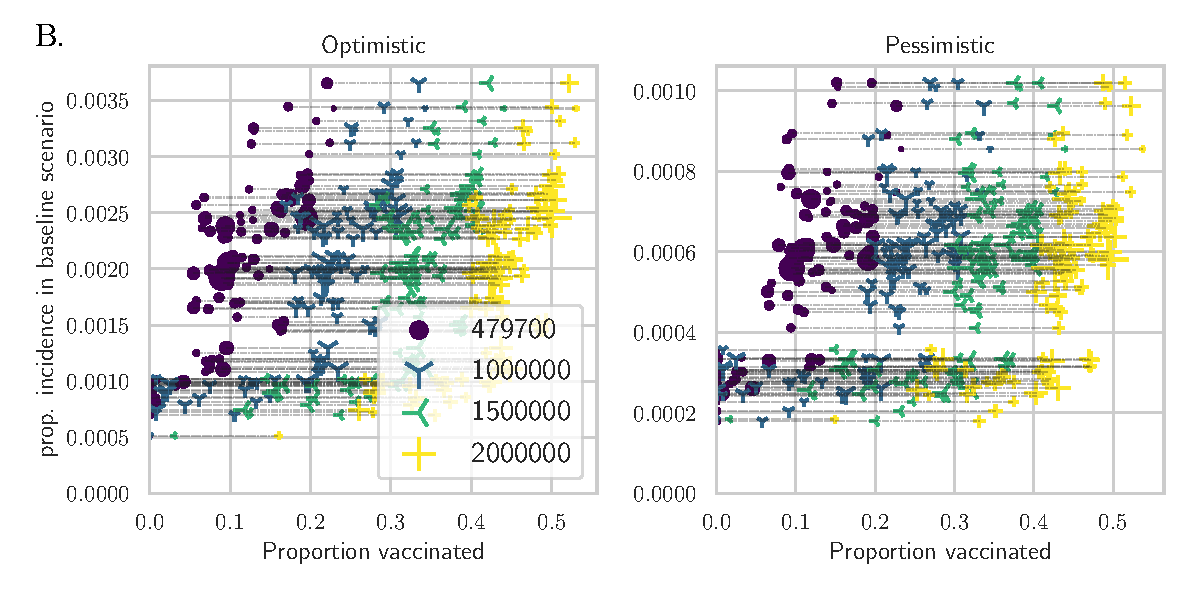
\includegraphics{fig_italy-ocp/figures/scatter_scn.pdf}
\caption[Analysis of the optimal solution]{Analysis of the optimal solution. A. Vaccinated population according to the optimal strategy against the projected incidence without vaccination, both normalized by provincial population size and considering the scenario with a weekly stockpile delivery of 479'700 doses. B. Same as in A, but considering all four scenarios of weekly stockpile replenishment. Each dot represents a province, with dot size proportional to its population.}
    \label{fig:OC_scatter}
\end{figure}


%% ***********************************************************************************************
\section{Discussion and Conclusion}
%% ***********************************************************************************************
Without any constraint on supply, each country would vaccinate its population as fast as possible according to the available infrastructure. However limitations in vaccine supply and rate of delivery are a reality for every country, hence the available doses should be deployed in space and time following a fair and effective strategy. 

In stockpile-limited settings, like most current vaccination campaigns worldwide, careful allocation may significantly increase the number of averted infections and deaths. The goal is to distribute the vaccines where they have the strongest beneficial impact on the dynamics of the epidemic. However, deriving an algorithm capable of computing spatially optimal allocation strategies in real, heterogeneous settings is far from trivial and our approach is, to the best of our knowledge, the first attempt in this direction. 

An novel optimal control framework has been developed, that delivers the best vaccination strategy under constraints on supply and logistics. This allows us to compute the allocation strategy that maximizes the number of averted infections during a projection of the COVID-19 epidemic in Italy from January 11, 2021 to April 11, 2021. Our results show that the optimal strategy has a complex structure that mainly reflects the projected incidence of each province, but also takes into account the spatial connectivity provided by the mobility network and the landscape of acquired population immunity. Although the reason why this strategy is optimal is not immediately intuitive, our simulations clearly outline its better overall performances over other, more straightforward strategies. This comparison suggests that the simplicity underlying intuitive vaccination strategies may undermine their effectiveness, and calls for complementing these simple approaches with rigorous and objective mathematical tools, like optimal control, that allow a full account of the complexity of the problem.

The present work demonstrate that it is possible to solve optimal control problems for spatially explicit dynamical models of infectious diseases at a national scale, thus overcoming the computational limitations that, up to now, precluded this kind of applications. The proposed framework can account for any compartmental epidemic model, with up to hundreds of connected spatial nodes. Supply and logistic constraints can be adapted to the actual landscape of decisions faced by the stakeholders, such as no/reduced vaccine delivery on weekends, or the need for fairness in vaccine distribution, e.g. by ensuring that each region receives at least a fixed fraction of the available vaccines. This is especially important as in our optimal allocation scenarios, some provinces receive no vaccine at all. Moreover, the optimization can be carried for single-dose vaccines, as done here, or for two-dose vaccines, where one could potentially optimize the time between the first and second dose (and if a second dose should be administered at all), clearly also considering the intervals recommended by the health authorities.

% Limitations
The method developped is obviously not devoid of limitations. The main one is that the optimal vaccination strategy strongly depends on the projection of the underlying epidemiological model. These projections are subject to several sources of uncertainty, especially for long term horizons, for example due to model design and calibration\cite{Cramer:EvaluationIndividualEnsemble:2021}, the generation of baseline transmission scenarios, and unforeseen events that may change the course of the epidemic (such as the importation of cases, the emergence of new virus variants, changes in disease awareness or social distancing policies). The optimal vaccination strategy is thus reliable only if the projections given by the underlying model dynamics are sufficiently accurate. A successful approach developed by the automatic control community to tackle that issue, named Model Predictive Control~\cite{Rawlings:ModelPredictiveControl:2017}, consists in compensating the performance losses expected over long horizons by constantly adapting the optimal strategy. In this context, Model Predictive Control might be implemented using the following steps: (a) at the beginning of each week, the state of the system is estimated by using newly acquired epidemiological data; (b) the optimization problem is solved over a fixed prediction horizon using the estimated state as initial condition; (c) the optimal strategy for the first week is applied and, as soon as the next weeks starts, these steps are repeated starting from (a). This method corrects the model inaccuracies by constantly resetting the initial state to the estimated one. Moreover, constraints may be updated to account for unexpected deliveries or new orders. Future work will aim at further evaluating the benefits of implementing this scheme for the design of optimal vaccination strategies.

Moreover, the epidemiological model underlying our control optimization has known validity and limitations\cite[-3\baselineskip]{Gatto:SpreadDynamicsCOVID19:2020, Bertuzzo:GeographyCOVID19Spread:2020}. An additional limitation of the model for the specific scopes of this work is that it does not account explicitly for risk-based classes, and thus does not account for the heterogeneities that may result from the demography of the population, as well as from the age-related transmission and clinical characteristics associated with COVID-19. While surely limiting for operational use of the tools, the scope of this \textsc{Chapter} is to provide a proof-of-concept of the relevance of spatial effects, which have not been addressed so far in the literature. To that end, our results support the relevance of the research question posed. Our framework can anyway be extended to optimize across both spatial and risk heterogeneities. 

A counter-factual assumption in this work is tha a one-dose vaccine with full and instantaneous efficacy against transmission is considered. At the time of development, the details about COVID-19 vaccines were not released, and this hypothesis allowed us to demonstrate our framework in a simple setting. Our framework can be further extended to account also for the simultaneous deployment of different vaccine types, some of which may require the administration of two doses. This extension too is subject of ongoing research, in particular to extend the modeling tools described here to accommodate the peculiarities of each authorized vaccine candidate while designing effective spatiotemporal deployment strategies.

% Conclusion
In conclusion, in this work the vaccine allocation at country scale has been optimized on different scenarios of epidemic transmission and vaccine availability. A spatially explicit compartmental model that had already been successfully used to describe the COVID-19 pandemic in Italy is updated using a data assimilation scheme. Then, the model is  discretized, transformed and simplified and a pipeline is constructed to perform large-scale nonlinear optimization on vaccine allocation, subject to stockpile and logistic constraints. Solving this problem yielded a complex solution that outperforms other strategies by a significant margin and proves robust across posterior realizations of the underlying model. As such, beside inherent limitations, it provides a benchmark against which other, possibly simpler vaccine rollout strategies can be usefully compared.

